\chapter[Small-Scale Environment]{The Influence of the Small-Scale Environment on Dwarf Galaxy Evolution}\label{ch:smallScaleEnvironment}


This work was done in collaboration with Daniele Schneider for her senior thesis 
``The effects of small-scale environment on dwarf galaxies.''


%%%%%%%%%%%%%%%%%%%%%%%%%%%%%%%%%%%%%%%%%%%%%%%%%%%%%%%%%%%%%%%%%%%%%%%%%%%%%%%%
%%%%%%%%%%%%%%%%%%%%%%%%%%%%%%%%%%%%%%%%%%%%%%%%%%%%%%%%%%%%%%%%%%%%%%%%%%%%%%%%


\section{Introduction}

%% Large-scale environment influence
%Large galaxy redshift surveys have shown that the large-scale structure of the 
%distribution of galaxies in the universe is similar to that of a 
%three-dimensional cosmic web \citep{Bond96}, where galaxy clusters are connected 
%by thin filaments of galaxies and are separated by voids (large, underdense 
%regions that occupy close to 60\% of space).  Over the last few decades, the 
%Sloan Digital Sky Survey \citep{Abazajian09,Ahn12} has accelerated the research 
%into the influence of the large-scale environment on the formation and evolution 
%of galaxies.
%
%Because gravitational clustering within a void proceeds as if in a very 
%low-density universe, cosmic voids are an important environment for studying 
%galaxy formation \citep[see][for a review]{vandeWeygaert11}.  The $\Lambda$CDM 
%cosmology predicts that galaxies formed in voids have lower masses and are 
%retarded in their star formation when compared to those in more dense 
%environments \citep{Gottlober03,Goldberg05,Cen11}.  The effects of the void 
%environment should be most obvious in dwarf galaxies due to their minimal 
%gravitational potential.  As a result, they are more sensitive to astrophysical 
%effects such as cosmological reionization, internal feedback from supernovae and 
%photoheating from star formation, small-scale details of dark matter halo 
%assembly, and the properties of dark matter.
%
%Observations have shown that the properties of dwarf galaxies vary dramatically 
%with the environment \citep[e.g.,][]{Ann08,Geha12}.  Void galaxies have been 
%found to have lower stellar mass \citep{Hoyle05,Croton05,Moorman15}, be bluer 
%and of a later type \citep{Grogin00,Rojas04,Patiri06,Park07,vonBendaBeckmann08,
%Hoyle12}, have higher star formation rates \citep{Rojas05,Moorman15,Beygu16}, 
%and be more gas rich \citep{Kreckel12,Moorman16,Jones16} than galaxies in denser 
%regions.

% Small-scale environment - what has been done so far?
In conjunction with the large-scale environment, the small-scale environment 
($\sim$1 \hMpc) has also been found to influence a galaxy's evolution.  A 
well-established morphology-density relation exists \citep{Dressler80}, where 
the fraction of late-type galaxies is inversely proportional to the local 
density.  \cite{Ellison09} determined that a galaxy's local environment 
influences a galaxy's evolution more than its large-scale environment.  
Likewise, \cite{Rupke08} concluded that interacting galaxies have suppressed 
metallicities because interactions induce flows of hydrogen.  For galaxies with 
$M_r < -19$, \cite{Park09} found that galaxy interactions out to the virial 
radius of the nearest neighbor influence the evolution of the target galaxy.  
Along with \cite{Park07}, they determine that the large-scale environment has a 
minimal effect on the evolution of a galaxy once the luminosity and morphology 
are taken into account.

We want to understand if the small-scale environment is more influential in a 
galaxy's evolution than its large-scale environment.  One important question 
within the small-scale environment asks if tidal influences due to the nearest 
neighbor galaxy or gravitational potentials from the nearest galaxy group are 
more influential in a galaxy's evolution.  A group consists of multiple galaxies 
that share the same dark matter halo.  A group member will interact 
gravitationally with all other group members, not just its nearest neighbor.  In 
groups and clusters dense enough to strip and heat the gas, galaxies will also 
experience ram pressure stripping.  And a galaxy near a group, but not within 
it, may also experience strong tidal effects from the group similar to and 
stronger than those from a neighboring galaxy.



%%%%%%%%%%%%%%%%%%%%%%%%%%%%%%%%%%%%%%%%%%%%%%%%%%%%%%%%%%%%%%%%%%%%%%%%%%%%%%%%
%%%%%%%%%%%%%%%%%%%%%%%%%%%%%%%%%%%%%%%%%%%%%%%%%%%%%%%%%%%%%%%%%%%%%%%%%%%%%%%%


\section[Nearest neighbor calculations]{Identifying the nearest neighbor}\label{sec:Theory_dist}

We employ two different spatial metrics to determine the best way to locate a 
galaxy's nearest neighbor.  We set a maximum velocity separation of 300 km/s 
between a galaxy and its nearest neighbor to capture the majority of interacting 
galaxies \citep[according to the distribution in peculiar velocity shown in][]
{Hwang10}.  Within a relative velocity $v_{rel} < 300\text{ km/s}$, we use 
either the physically closest galaxy in units of \hMpc or the galaxy within the 
smallest fraction of its virial radius; both these methods are described below 
in further detail.  The two methods result in different neighboring galaxies for 
about 46\% of our dwarf galaxy sample.


\subsection{Peculiar velocity}
% Finger of God

A galaxy's redshift is composed of both the expansion of the universe and the 
galaxy's peculiar velocity (its motion relative to the surrounding galaxies and 
environment).  Known as the ``Finger of God'' effect, the peculiar velocity 
causes galaxy groups and clusters to appear extended along the line of sight 
when using redshift as a distance measurement.  When we calculate distances on 
large scales, the peculiar velocity is negligible.  However, when we study the 
distance between two objects in the universe on a small scale (within a few 
\hMpc), the peculiar velocity dominates.  The relative velocity $v_{rel}$ 
between galaxies $a$ and $b$ is defined as
\begin{equation}
    v_{rel} = |z_a - z_b|c
\end{equation}
where $z$ is the redshift.  We require all 
neighbors to have a maximum relative velocity $v_{rel} < 300\text{ km/s}$, as we 
believe those outside this range will have minimal influence on the target 
galaxy's evolution.  We show in Sec. \ref{sec:selection_effects} that our 
results are insensitive to this value.


\subsection{Sky separation in \hMpc}

The distance on the sky between two galaxies is found by projecting the two 
galaxies onto a sphere of radius $\bar{r}$, where $\bar{r}$ is the average 
distance from Earth of the two galaxies.  This assumes that two galaxies which 
are gravitationally bound are in a system where the relative velocity between us 
and the system is 0 and that $\bar{r}$ is the distance to the center of the 
system.  For redshifts $z \ll 1$, we can approximate the distance to the system 
as
\begin{equation}
    \bar{r} = \frac{\bar{z}c}{H_0}
\end{equation}
where $\bar{z}$ is the average redshift of the two galaxies, $c$ is the speed of 
light, and $H_0$ is the Hubble constant.  Each galaxy's right ascension (RA) and 
declination (dec.) are converted to Cartesian coordinates to find their sky 
separation.


\subsection{Fractional virial radii}
% Virial radius calculation

The virial radius of a galaxy defines the region within which something is 
gravitationally bound to the galaxy.  From \cite{Hwang10}, we calculate the 
virial radius of a galaxy to be
\begin{equation}\label{eqn:r_vir}
    r_{vir} = (3L\gamma/4\pi/200\rho_c)^{1/3}
\end{equation}
where $L$ is the galaxy's luminosity, $\gamma$ is the mass-to-light ratio, and 
$\rho_c$ is the critical density of the universe.  The critical density is the 
density at which evenly distributed gas would collapse to form a galaxy.  

\cite{Choi07} find that the velocity dispersion of a galaxy depends on its 
morphological type, where $\sqrt{2}\sigma_{late} \approx \sigma_{early}$.  In 
terms of the velocity dispersion, the kinetic energy of a galaxy 
$K = 3/2 \sigma^2$.  Its gravitational potential energy $U = 3GM/5R$.  
Therefore, the virial theorem shows us that
\begin{align}
    3\sigma^2 \simeq \frac{3}{5} \frac{GM}{R}\nonumber \\
    M \simeq \frac{5\sigma^2 R}{G}
\end{align}
With $\gamma \equiv M/L$, at a fixed luminosity and virial radius we see that
\begin{equation}
    \gamma_{late} \simeq \frac{5\sigma_{late}^2 R}{GL} \qquad \gamma_{early} \simeq \frac{5\sigma_{early}^2 R}{GL}
\end{equation}
Taking the ratio of the two mass-to-light ratios and using the relation between 
the velocity dispersions found by \cite{Choi07}, we find that the mass-to-light 
ratio depends on the galaxy's morphological type: 
$\gamma_{early} = 2\gamma_{late}$.

\cite{Hwang10} define $200\rho_c = 740\bar{\rho}$, where 
$\bar{\rho} = (0.0223\pm 0.0005)(\gamma_{late}L_{-20})(\text{\hMpc})^3$.  We can 
then rewrite Eqn. \ref{eqn:r_vir} as
\begin{equation}
    r_{vir} = \left( \frac{3}{4\times 740\times 0.0223\pi} \frac{\gamma}{\gamma_{late}} \frac{L}{L_{-20}} \right)^{1/3}
\end{equation}
where $L_{-20}$ is the luminosity of a galaxy with $M_r = -20$.  We can then use 
the virial radius to scale the distance between two galaxies as a fraction of 
the neighbor's virial radius.

Rather than using a measure of the virial radius for the group analysis, we 
scale the distance as a fraction of the group's root mean square (rms) radius.


\subsection{Absolute distance to nearest neighbor}
% Including redshift

We can also calculate the distance between two galaxies by ignoring the effects 
of their relative velocities.  Instead of projecting both galaxies onto a sphere 
with radius $\bar{r}$, we instead project each onto its own sphere of radius 
\begin{equation}
    r = \frac{cz}{H_0}
\end{equation}
(This approximation for the distance is valid because all our target galaxies 
are within a redshift $z \leq 0.03$.)  We then convert to Cartesian coordinates 
and use the three-dimensional Pythagorean theorem to calculate the distance 
between the two galaxies.


%%%%%%%%%%%%%%%%%%%%%%%%%%%%%%%%%%%%%%%%%%%%%%%%%%%%%%%%%%%%%%%%%%%%%%%%%%%%%%%%
%%%%%%%%%%%%%%%%%%%%%%%%%%%%%%%%%%%%%%%%%%%%%%%%%%%%%%%%%%%%%%%%%%%%%%%%%%%%%%%%


\section[SDSS Data]{SDSS Data and galaxy selection}

% SDSS
%The Sloan Digital Sky Survey Data Release 7 \citep[SDSS DR7;][]{Abazajian09} is 
%a wide-field multiband imaging and spectroscopic survey which maps approximately 
%one-quarter of the northern sky using a drift scanning technique.  Photometric 
%data in the five-band SDSS system --- $u$, $g$, $r$, $i$, and $z$ --- is taken 
%on a dedicated 2.5m telescope at the Apache Point Observatory in New Mexico 
%\citep{Fukugita96,Gunn98}.  Galaxies with Petrosian $r$-band magnitudes 
%$m_r < 17.77$ are selected for follow-up spectroscopic analysis \citep{Lupton01,
%Strauss02}.  The galaxy colors are taken from the Korean Institute for Advanced 
%Study Value-Added Galaxy Catalog \citep[KIAS-VAGC;][]{Choi10}, which contains 
%galaxies from the SDSS DR7 main sky survey based on the New York University 
%Value-Added Galaxy Catalog Data Release 7 \citep[NYU-VAGC;][]{Blanton05}.  Total 
%star formation rates (SFR) and total specific star formation rates (sSFR) are 
%from the MPA-JHU value-added catalog\footnote{Available at 
%\url{http://www.mpa-garching.mpg.de/SDSS/DR7/}}, calculated using the technique 
%described in \cite{Brinchmann04}.  
The gas-phase chemical abundances used are from \cite{Douglass17c}, which are 
calculated using the Direct $T_e$ method.  The galaxies' large-scale 
environments are based on the void catalog compiled by \cite{Pan12}, which is 
constructed from SDSS DR7 using the VoidFinder algorithm of \cite{Hoyle02}.  
Galaxies that are located within identified voids are labeled as void galaxies, 
and those that do not fall within a void are designated as wall galaxies.  The 
large-scale environment within 5 \hMpc of the edge of the main SDSS DR7 
footprint cannot be described using the VoidFinder algorithm because the minimum 
diameter of a void is 10 \hMpc.  Therefore, the large-scale environment for 
galaxies within 5 \hMpc of the edge of the main footprint in SDSS DR7 is 
designated as unknown.

% photometry from KIAS-VAGC
% sSFR from MPA-JHU (Brinchmann04)
% gas-phase chemical abundances from Douglass17c


\subsection{Various samples}

% Spectroscopic sample (those with chemical abundance estimates)
% Full SDSS dwarf galaxy sample

Two galaxy samples are used in this analysis.  The largest one contains the 
11,002 dwarf galaxies spectroscopically observed in SDSS DR7.  The second sample 
contains those star-forming dwarf galaxies from the first set that have 
gas-phase chemical abundances in \cite{Douglass17c}, totaling 1920 dwarf 
galaxies.  Because this subset of galaxies contains only star-forming galaxies 
and is not representative of all dwarf galaxies, we show in Section 
\ref{sec:selection_effects} that this selection effect may affect our results.


\subsection{Group catalog}

In addition to comparing the target galaxies to their nearest neighbor, we also 
look at the relationship between the dwarf galaxies' properties and their 
proximity to the nearest galaxy group.  We use the \emph{Mr18} Berlind group 
catalog \citep{Berlind06} as our source of groups, which is built on the 
galaxies in the NYU-VAGC. The catalog identifies groups using a 
friends-of-friends algorithm \citep{Huchra82} to connect galaxies with 
$M_r < -18$.


%%%%%%%%%%%%%%%%%%%%%%%%%%%%%%%%%%%%%%%%%%%%%%%%%%%%%%%%%%%%%%%%%%%%%%%%%%%%%%%%
%%%%%%%%%%%%%%%%%%%%%%%%%%%%%%%%%%%%%%%%%%%%%%%%%%%%%%%%%%%%%%%%%%%%%%%%%%%%%%%%


\section[Analysis \& Results]{Distance analysis and results}

Our primary objective is to compare various physical characteristics of dwarf 
galaxies against their nearest neighbors or groups to discern how the 
small-scale environment affects their evolution.


\subsection{Parameter -- distance relations}\label{sec:Relations}

The relationships between various physical parameters and the distance to the 
nearest neighbor or group for our sample of star-forming dwarf galaxies are 
shown in Figs. \ref{fig:ur}--\ref{fig:NO}.  In each of the four plots within 
each figure, we bin the galaxies in distance-space and show the median parameter 
value in each bin, to discern any overall trends in the data.  We apply a linear 
regression to the data; the output of these fits are in Table \ref{tab:fits}.  
Each of these four plots probes the distance relationship from a different 
angle.  The top left plots in Figs. \ref{fig:ur}--\ref{fig:NO} relate the target 
dwarf galaxy's parameter to the distance to its nearest neighbor, as defined by 
the closest galaxy on the sky in \hMpc with a velocity difference less than 300 
km/s.  The bottom left plots relate the target dwarf galaxy's parameter to the 
distance to its nearest neighbor, as defined by the closest galaxy on the sky in 
units of the virial radius of the neighbor galaxy with a velocity difference 
less than 300 km/s.  The nearest galaxy is not necessarily the same for these 
two distance measurements, as explained in Sec. \ref{sec:Theory_dist}.

We repeat this same analysis on the nearest group to the target dwarf galaxy.  
The top right plots in Figs. \ref{fig:ur}--\ref{fig:NO} relate the target dwarf 
galaxy's parameter to the distance to the center of the nearest group, as 
defined as the closest group in the sky in \hMpc with a velocity difference less 
than 300 km/s.  The bottom right plots in Figs. \ref{fig:ur}--\ref{fig:NO} 
relate the target dwarf galaxy's parameter to the distance to the nearest group 
as defined by the closest group on the sky in units of the group's rms radius 
with a velocity difference of less than 300 km/s.  Groups are very rare in voids 
(by nature of the void environment), so the uncertainty in the binned values 
shown in these plots is much larger than in the galaxy neighbor plots.

These figures reveal influences from both the large-scale and small-scale 
environments, since we are identifying which galaxies reside in void regions and 
which do not.


\subsubsection{Color}

\begin{figure}
    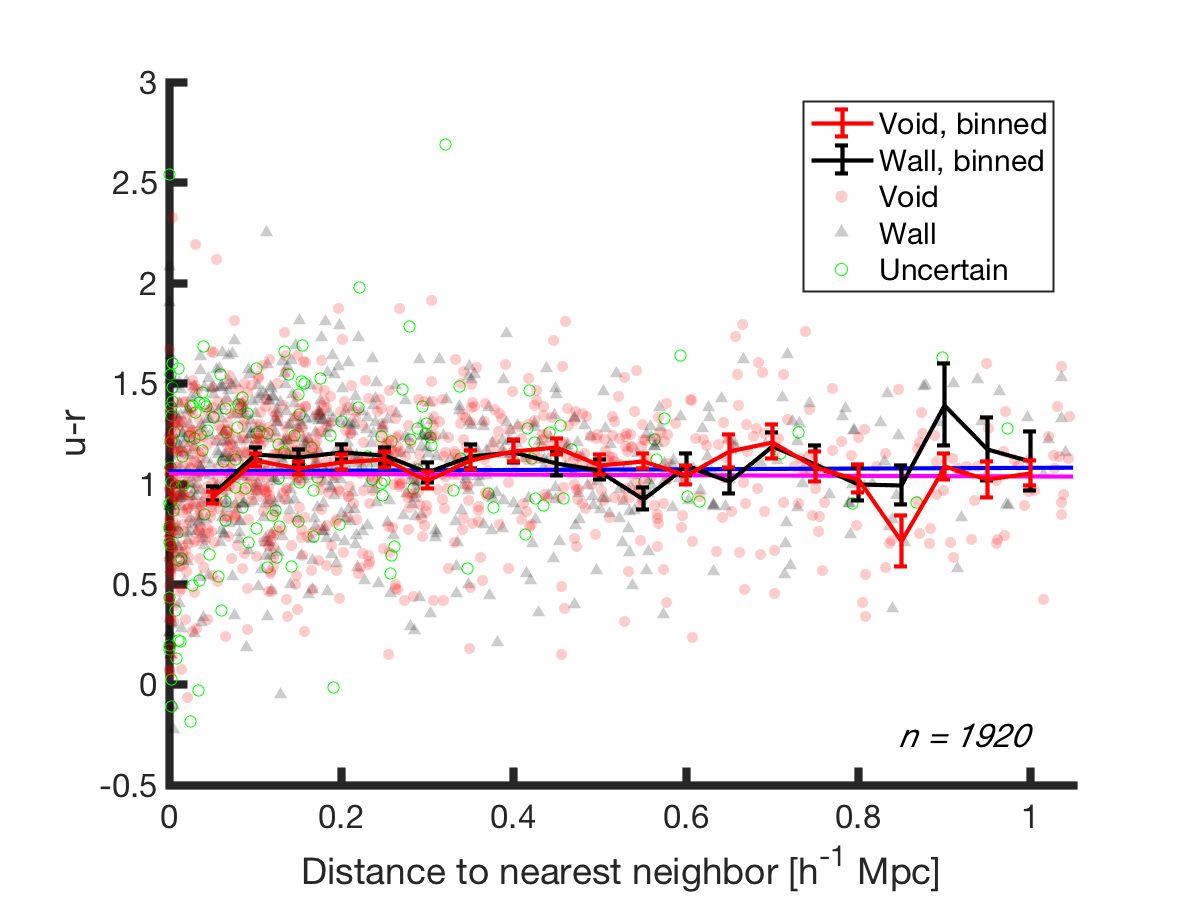
\includegraphics[width=0.49\textwidth]{Images/smallScaleEnvironment/1sig_dwarf_I06relations_absDist_ur}
    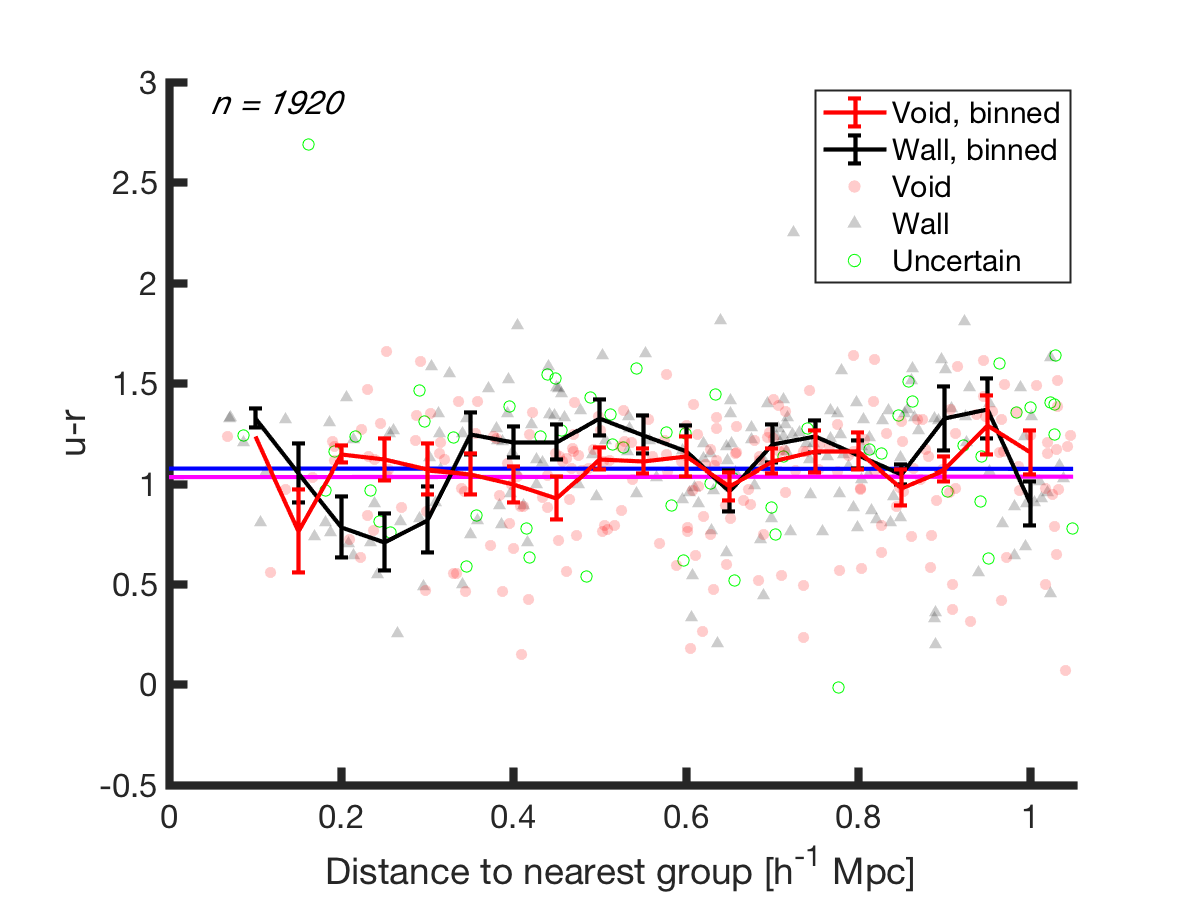
\includegraphics[width=0.49\textwidth]{Images/smallScaleEnvironment/1sig_dwarf_I06relations_groupAbsDist_ur}
    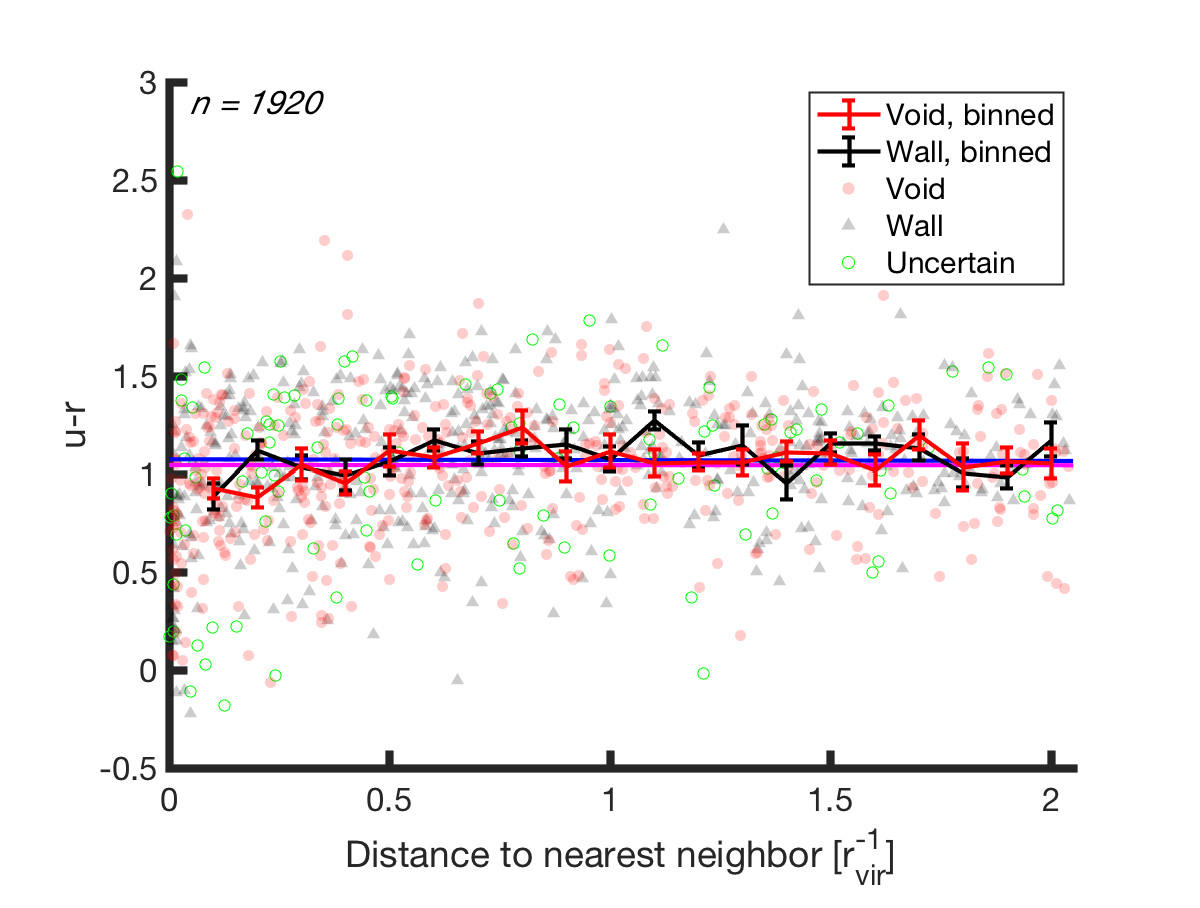
\includegraphics[width=0.49\textwidth]{Images/smallScaleEnvironment/1sig_dwarf_I06relations_virDist_ur}
    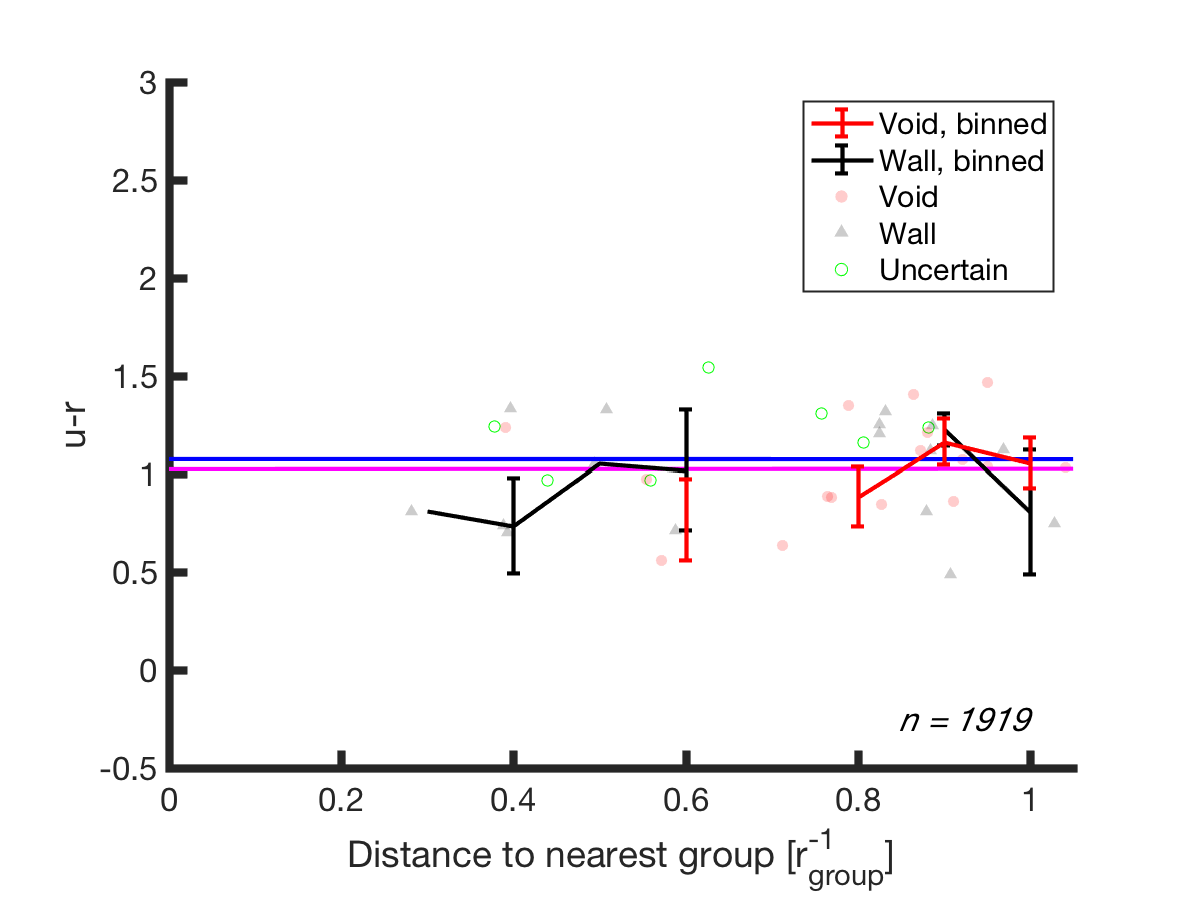
\includegraphics[width=0.49\textwidth]{Images/smallScaleEnvironment/1sig_dwarf_I06relations_groupRDist_ur}
%    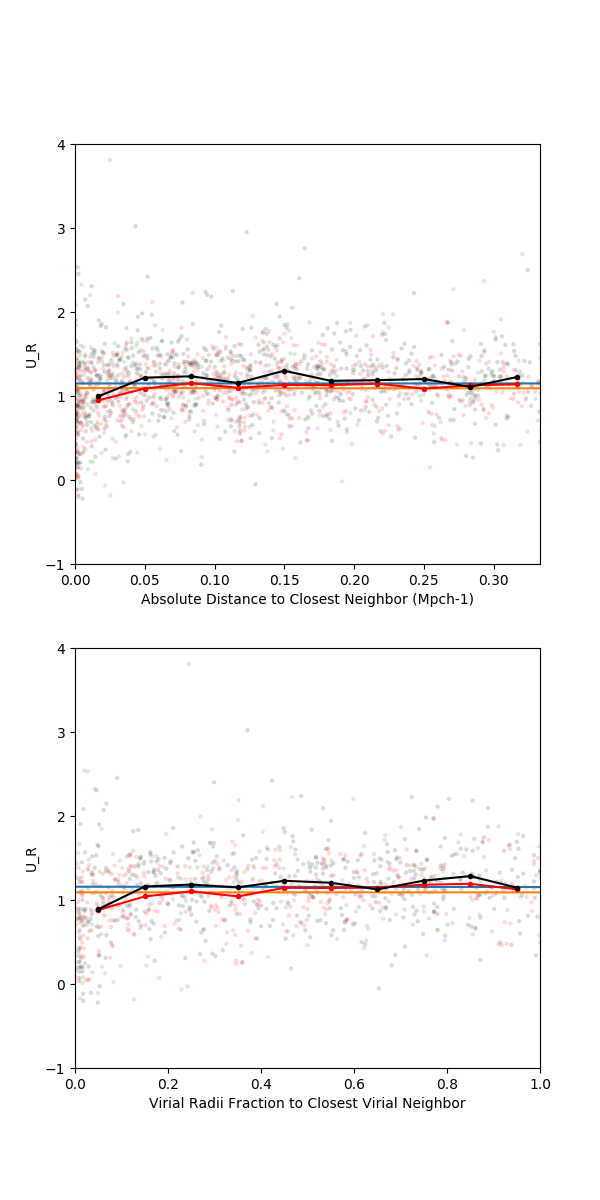
\includegraphics[width=0.49\textwidth]{Images/smallScaleEnvironment/dwarf_ur_300}
%    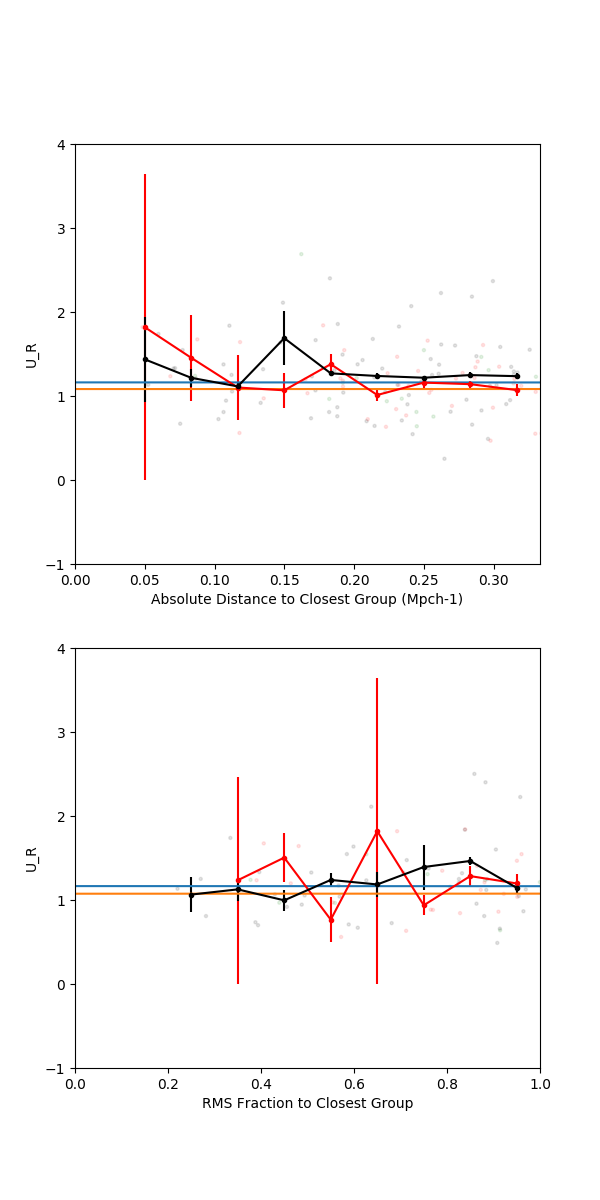
\includegraphics[width=0.49\textwidth]{Images/smallScaleEnvironment/dwarf_ur_300_group}
    \caption[$u-r$ versus distance to nearest neighbor and group]{Color ($u-r$) 
    versus distance to the nearest galaxy (on the left) and nearest group (on 
    the right).  The top panels show the color as a function of the sky 
    separation in \hMpc between the target dwarf galaxy and the neighbor, while 
    the bottom panels show the color as a function of the closest virial 
    neighbor.  Void galaxies are shown in red, while wall galaxies are shown in 
    black and unknown in green.  We have also included the median color for the 
    galaxies after binning by distance, to discern any finer behavior in the 
    relationships.  Linear fits to the void and wall galaxies are shown in 
    orange and blue, respectively.  It is clear that the void dwarf galaxies are 
    bluer than the wall dwarf galaxies.  The nearest galaxies appear to only 
    have some affect on the dwarf galaxy's color at separations less than 0.05 
    \hMpc, or 0.1$r_{vir}$ (for wall galaxies; 0.2$r_{vir}$ for void galaxies).  
    There appears to be no relationship between a dwarf galaxy's color and its 
    distance to the nearest group.}
    \label{fig:ur}
\end{figure}

Because of the known morphology-density relation, we expect to find that a dwarf 
galaxy's color becomes bluer as the distance to the nearest group increases, but 
we expect the dwarf galaxy's color to become bluer as the distance to the 
neighboring galaxy decreases.  Fig. \ref{fig:ur} shows very little relationship 
between the distance and color, except in the smallest distance bin.  The linear 
fits quantify this observation --- the slopes are on the order of 10$^{-3}$.  
However, within a distance of 0.05 \hMpc or 0.1$r_{vir}$ (for wall galaxies; 
0.2$r_{vir}$ for void galaxies), dwarf galaxies tend to be bluer than at further 
distances from their nearest neighbor.  There does not appear to be any 
relationship between a dwarf galaxy's color and its distance to the center of 
the nearest group.  It has been well-established that void galaxies tend to be 
bluer than galaxies in denser environments \citep{Grogin99,Rojas04,Patiri06,
vonBendaBeckmann08,Hoyle12}; this shift is apparent in Fig. \ref{fig:ur}, where 
the void dwarf galaxies are slightly bluer than the wall dwarf galaxies at all 
distances.  


\subsubsection{Specific star formation rate}

\begin{figure}
    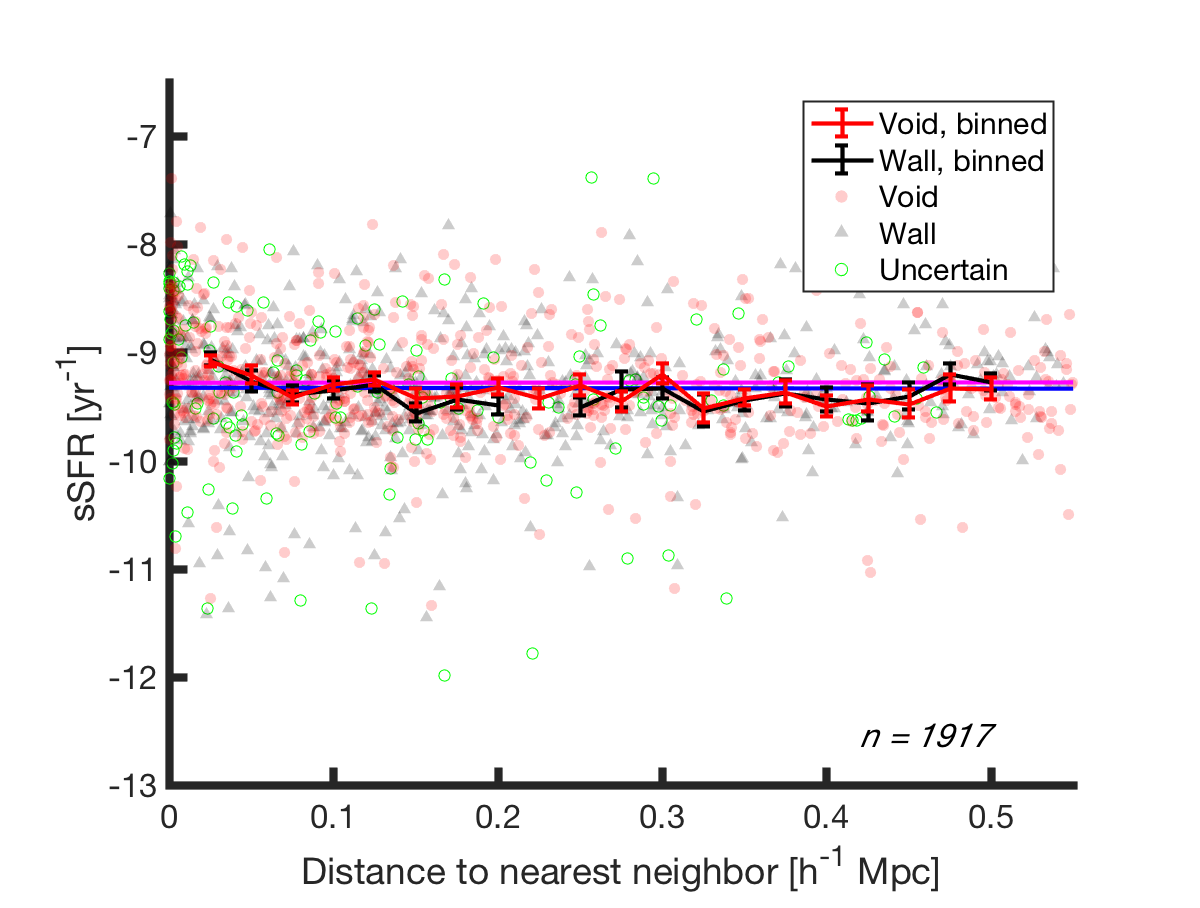
\includegraphics[width=0.49\textwidth]{Images/smallScaleEnvironment/1sig_dwarf_I06relations_absDist_sSFR}
    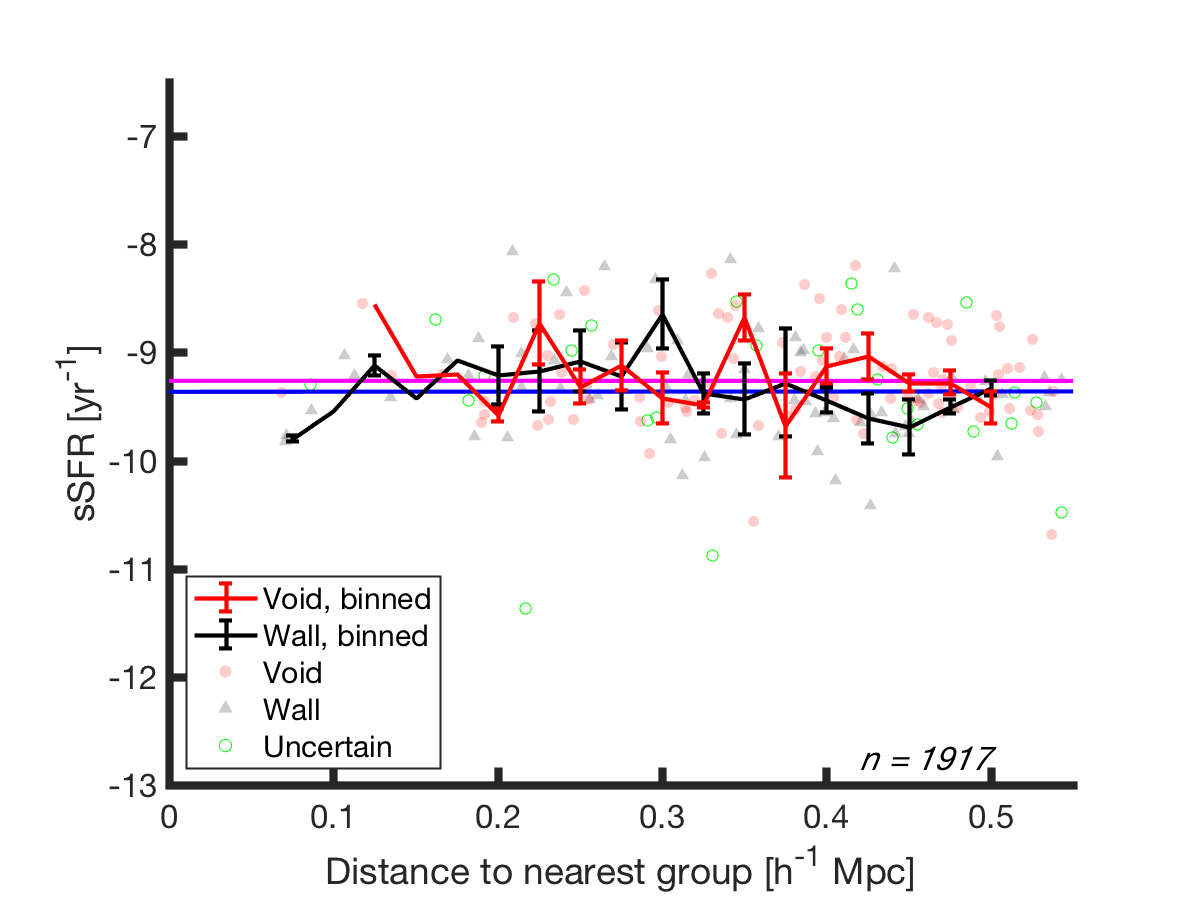
\includegraphics[width=0.49\textwidth]{Images/smallScaleEnvironment/1sig_dwarf_I06relations_groupAbsDist_sSFR}
    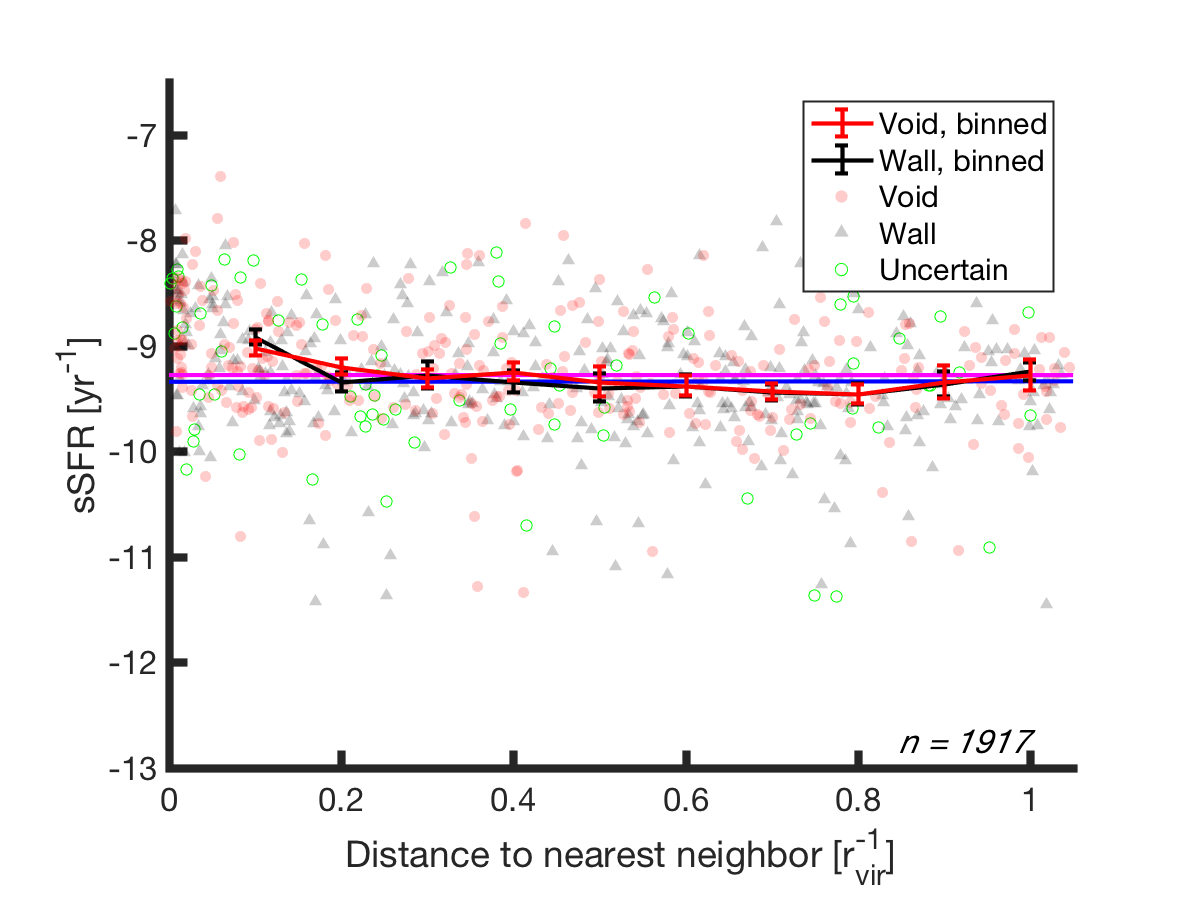
\includegraphics[width=0.49\textwidth]{Images/smallScaleEnvironment/1sig_dwarf_I06relations_virDist_sSFR}
    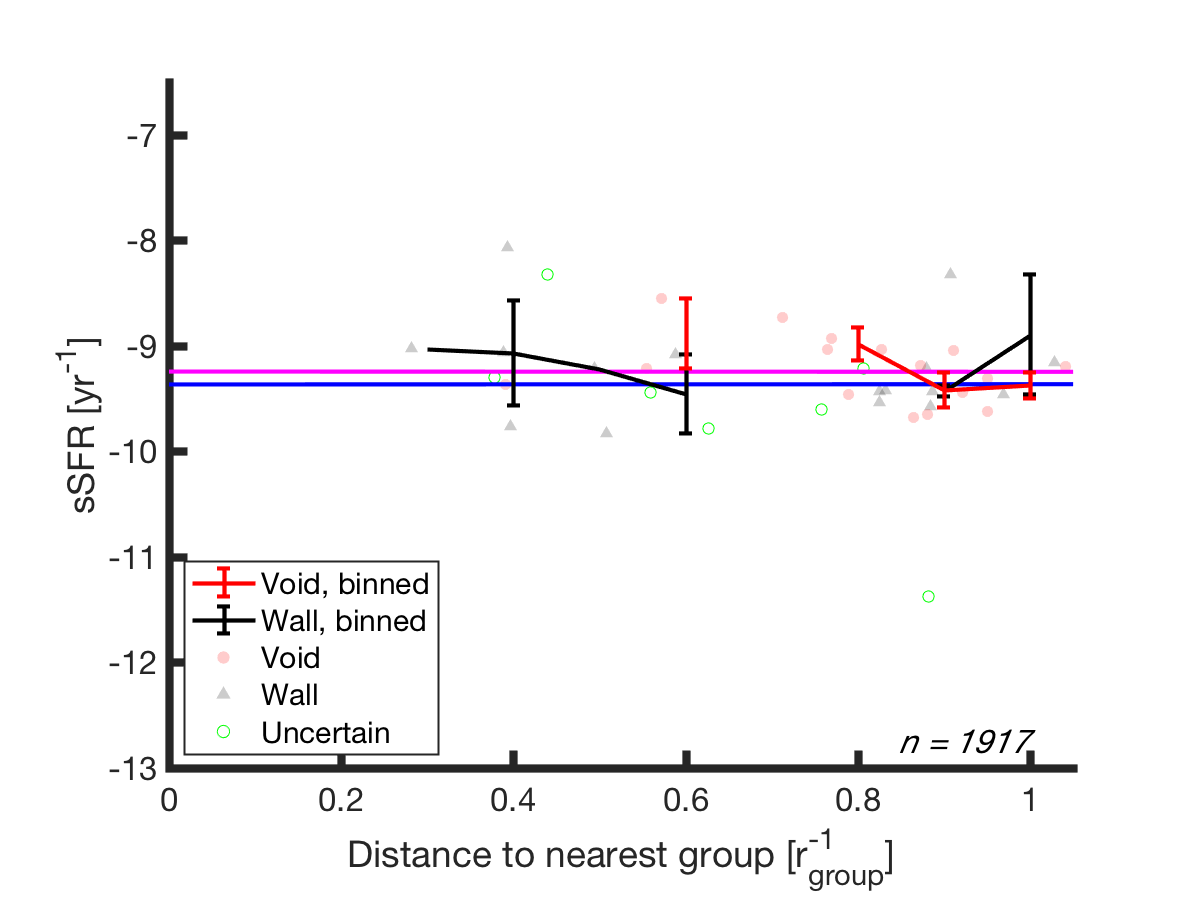
\includegraphics[width=0.49\textwidth]{Images/smallScaleEnvironment/1sig_dwarf_I06relations_groupRDist_sSFR}
%    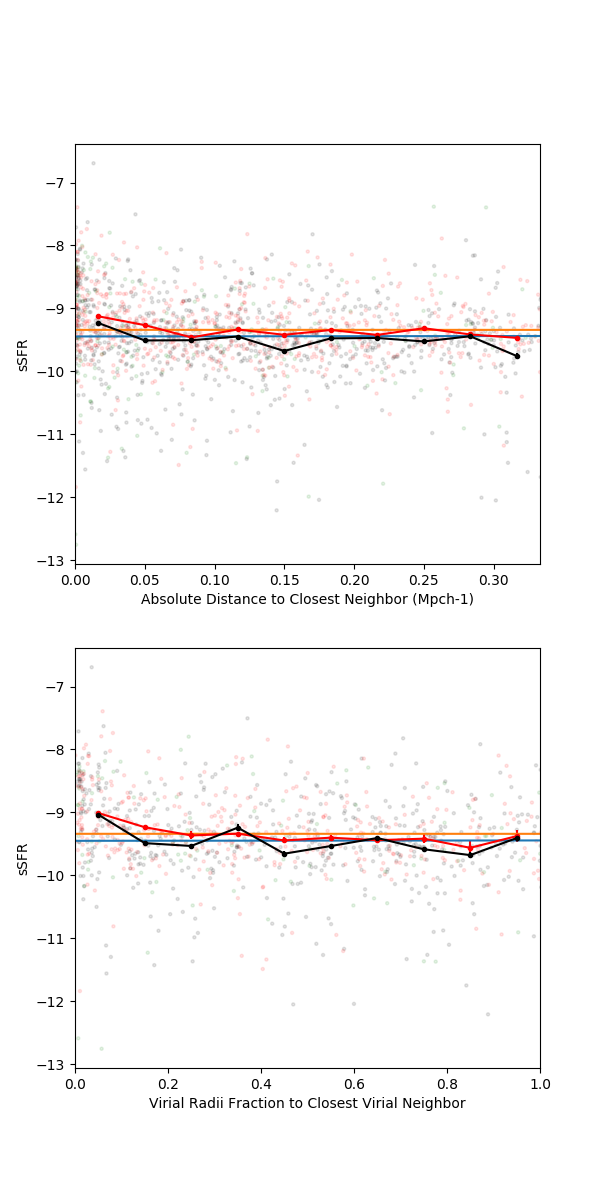
\includegraphics[width=0.49\textwidth]{Images/smallScaleEnvironment/dwarf_sSFR_300}
%    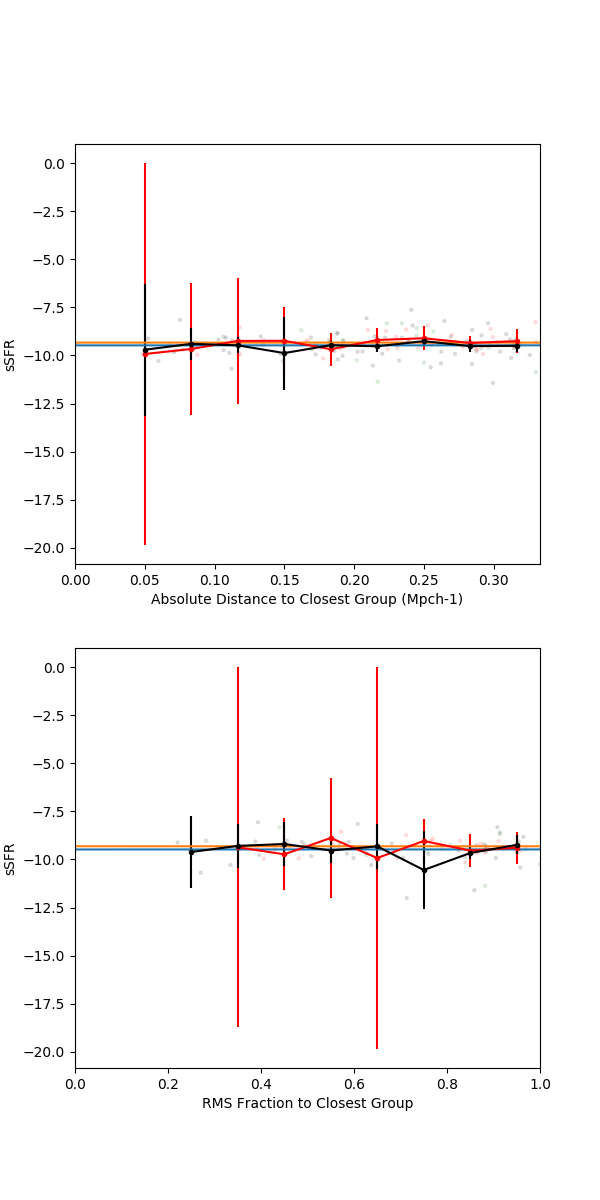
\includegraphics[width=0.49\textwidth]{Images/smallScaleEnvironment/dwarf_sSFR_300_group}
    \caption[sSFR versus distance to nearest neighbor and group]{sSFR versus 
    distance to the nearest galaxy (on the left) and nearest group (on the 
    right).  The top panels show the sSFR as a function of the sky separation in 
    \hMpc between the target dwarf galaxy and the neighbor, while the bottom 
    panels show the sSFR as a function of the closest virial neighbor.  Void 
    galaxies are shown in red, while wall galaxies are shown in black and 
    unknown in green.  We have also included the median sSFR for the galaxies 
    after binning by distance, to discern any finer behavior in the 
    relationships.  Linear fits to the void and wall galaxies are shown in 
    orange and blue, respectively.  It is clear that the void dwarf galaxies 
    have higher sSFRs than the wall dwarf galaxies.  Only the neighbor galaxies 
    at separations less than 0.05 \hMpc or 0.1$r_{vir}$ (for wall galaxies; 
    0.2$r_{vir}$ for void galaxies) appear to have some affect on the dwarf 
    galaxies' sSFR.  There appears to be no relationship between a dwarf 
    galaxy's sSFR and its distance to the nearest group.}
    \label{fig:sSFR}
\end{figure}

Following our prediction for the color-distance relations, we expect the 
specific star formation rate (sSFR) to decrease with distance from the nearest 
neighbor and increase with distance from the nearest group.  We also see very 
little relationship between the distance and sSFR in Fig. \ref{fig:sSFR}, except 
in the smallest distance bin.  The linear fits quantify this observation --- the 
slopes are on the order of 10$^{-3}$.  Within a distance of 0.05 \hMpc or 
0.1$r_{vir}$ (for wall galaxies; 0.2$r_{vir}$ for void galaxies), dwarf galaxies 
tend to have higher sSFRs than at further distances from their nearest neighbor.  
There does not appear to be any relationship between a dwarf galaxy's sSFR and 
its distance to the center of the nearest group in either distance metric.  In 
these distance comparisons, there is a shift towards higher sSFRs in the void 
dwarf galaxies when compared to the wall dwarf galaxies, as has been previously 
observed \citep{Rojas05,vonBendaBeckmann08,Moorman15,Beygu16}.  


\subsubsection{Metallicity}

\begin{figure}
    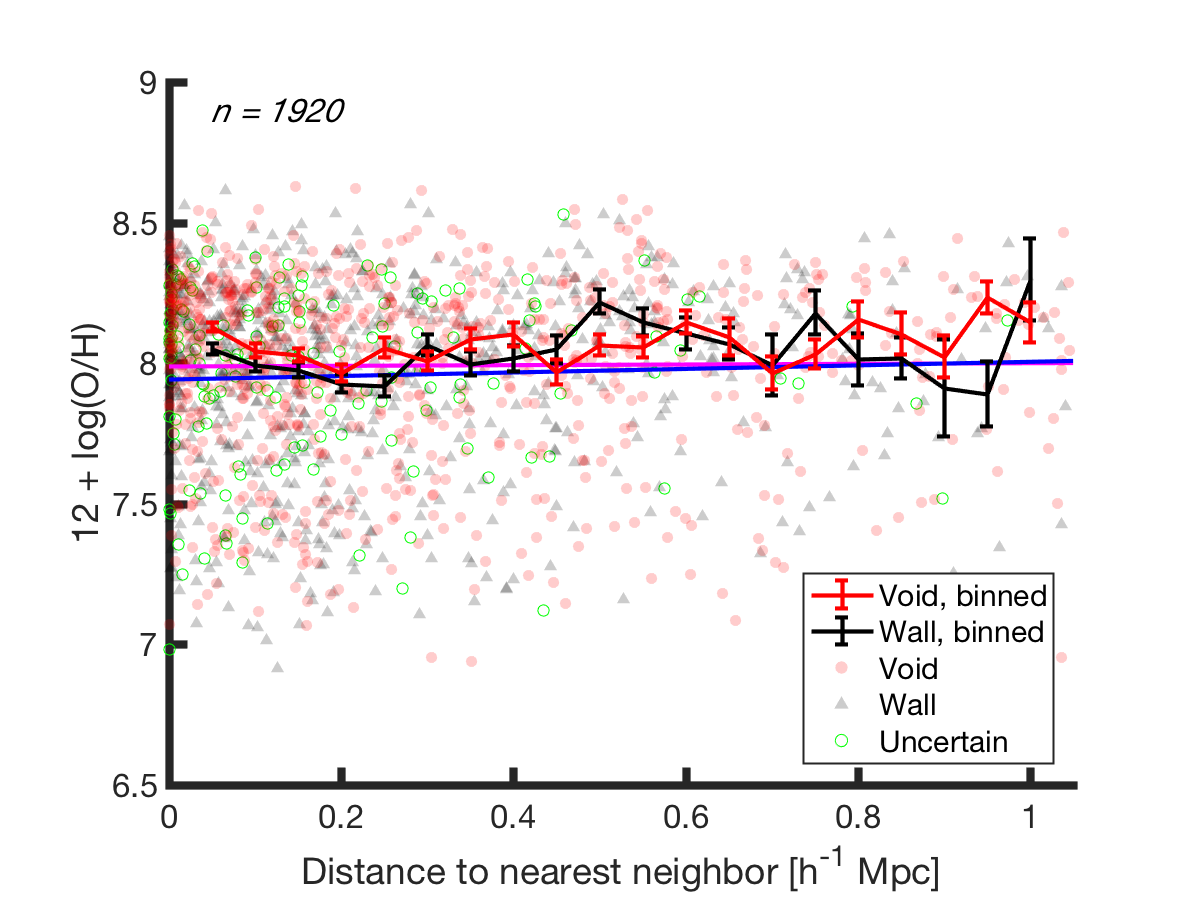
\includegraphics[width=0.49\textwidth]{Images/smallScaleEnvironment/1sig_dwarf_I06relations_absDist_OH}
    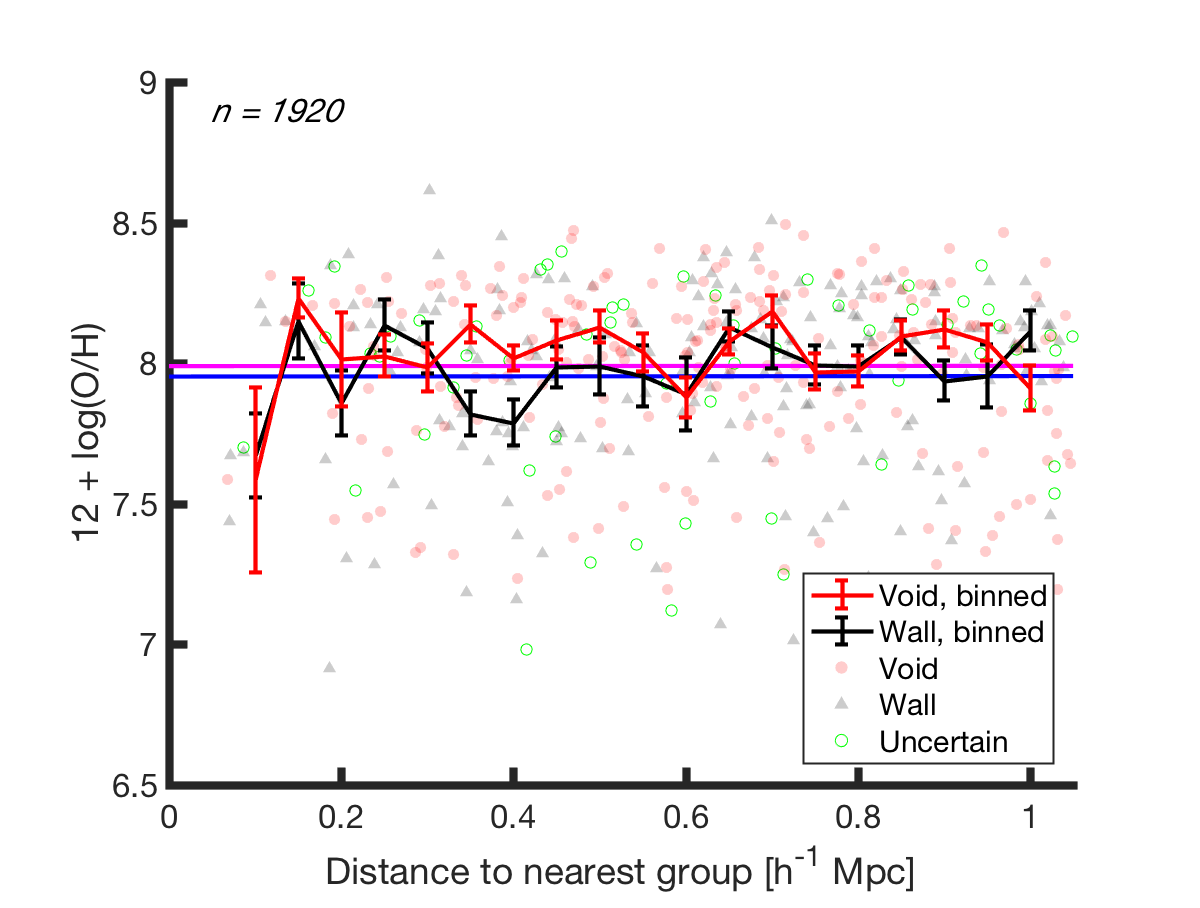
\includegraphics[width=0.49\textwidth]{Images/smallScaleEnvironment/1sig_dwarf_I06relations_groupAbsDist_OH}
    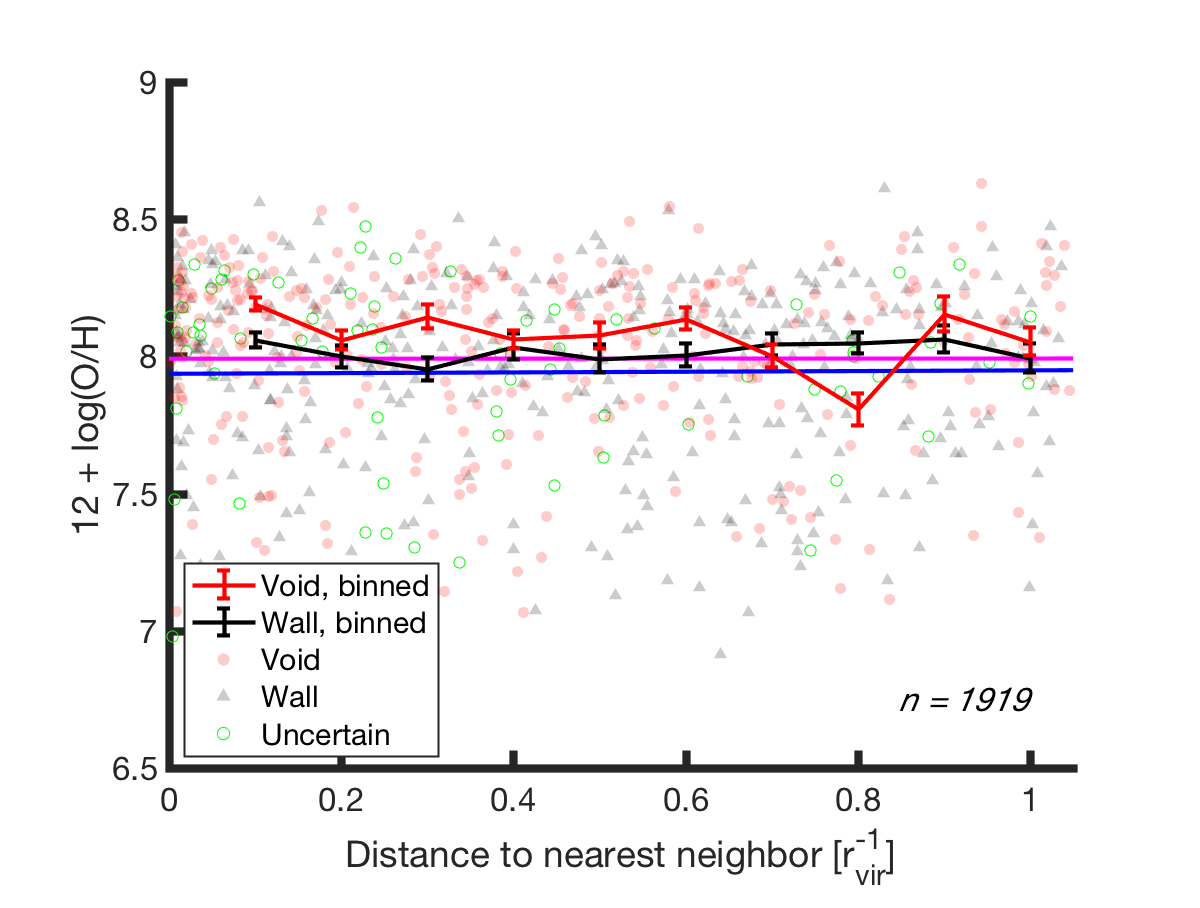
\includegraphics[width=0.49\textwidth]{Images/smallScaleEnvironment/1sig_dwarf_I06relations_virDist_OH}
    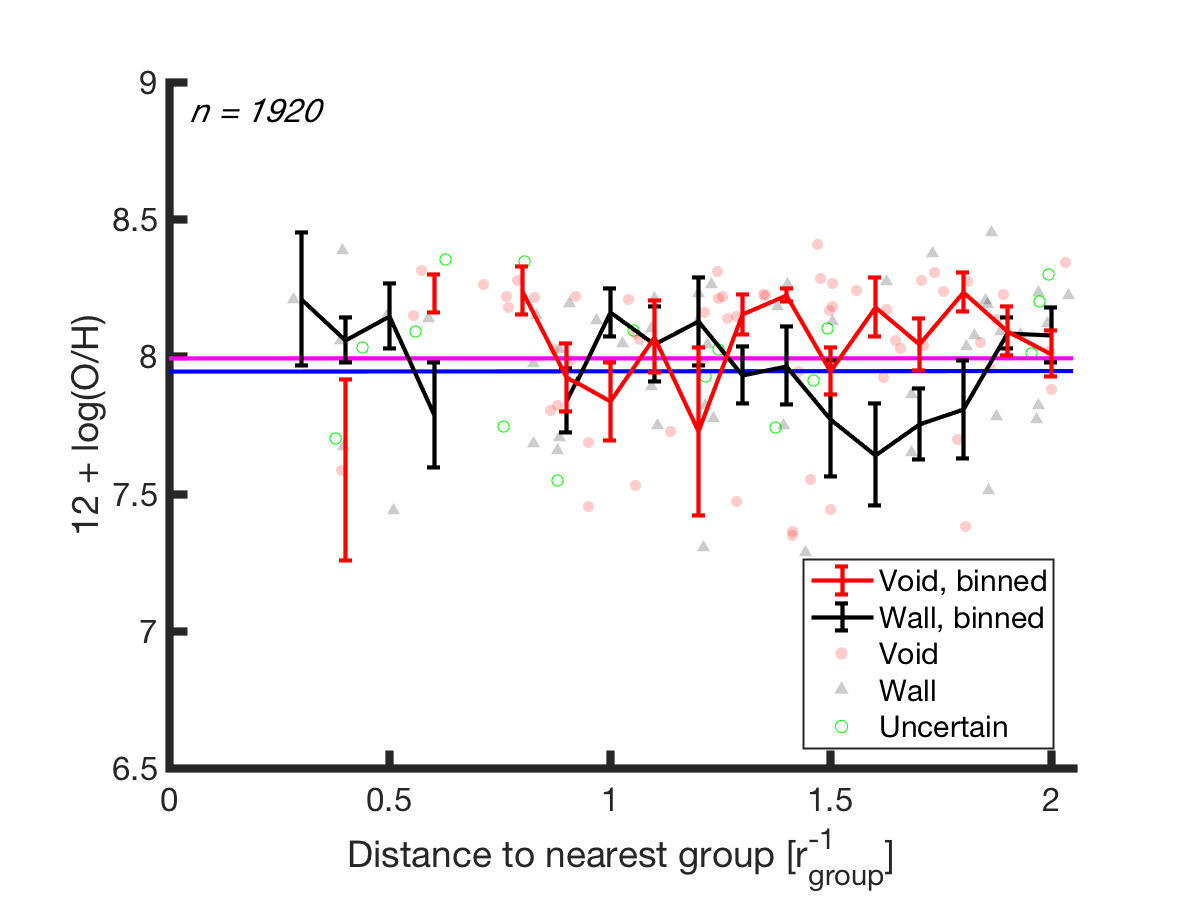
\includegraphics[width=0.49\textwidth]{Images/smallScaleEnvironment/1sig_dwarf_I06relations_groupRDist_OH}
%    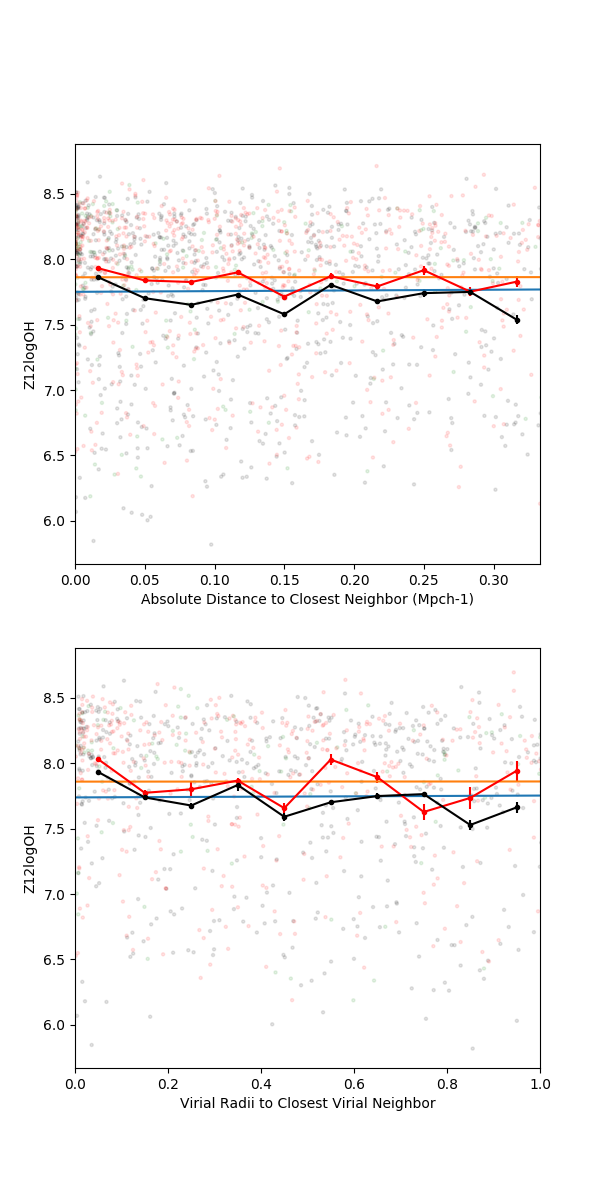
\includegraphics[width=0.49\textwidth]{Images/smallScaleEnvironment/dwarf_OH_300}
%    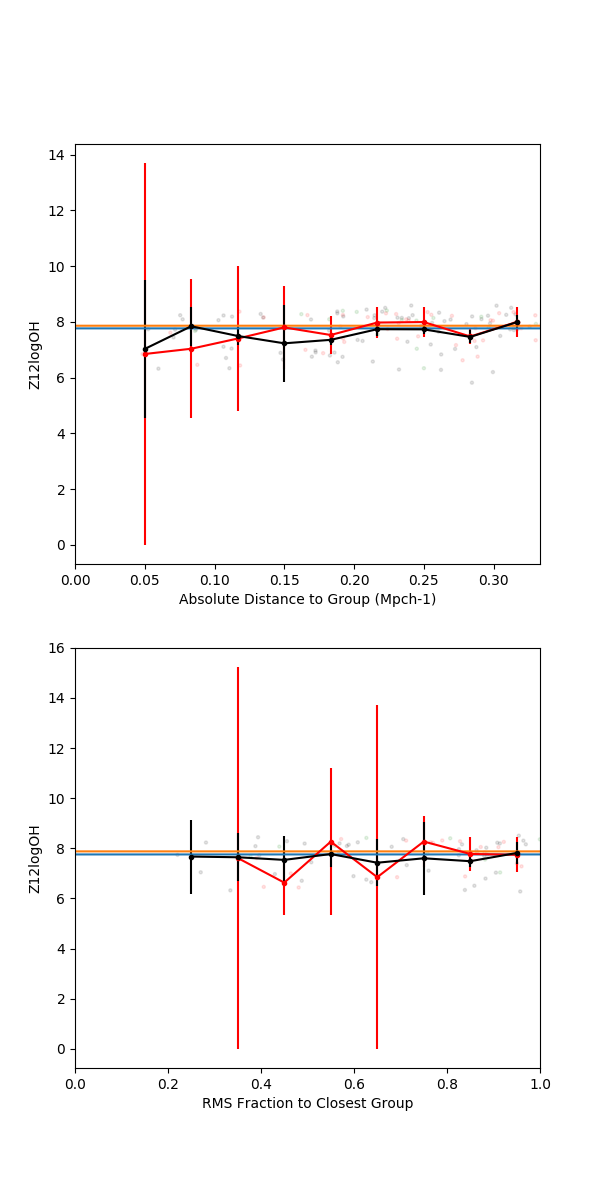
\includegraphics[width=0.49\textwidth]{Images/smallScaleEnvironment/dwarf_OH_300_group}
    \caption[Metallicity versus distance to nearest neighbor and group]
    {Metallicity versus distance to the nearest galaxy (on the left) and nearest 
    group (on the right).  The top panels show the metallicity as a function of 
    the sky separation in \hMpc between the target dwarf galaxy and the 
    neighbor, while the bottom panels show the metallicity as a function of the 
    closest virial neighbor.  Void galaxies are shown in red, while wall 
    galaxies are shown in black and unknown in green.  We have also included the 
    median metallicity for the galaxies after binning by distance, to discern 
    any finer behavior in the relationships.  Linear fits to the void and wall 
    galaxies are shown in orange and blue, respectively.  It is clear that the 
    void dwarf galaxies have higher metallicities than the wall dwarf galaxies.  
    Only the neighbor galaxies at separations less than 0.15 \hMpc appear to 
    have some affect on the dwarf galaxies' metallicity.  When measuring the 
    distance to the nearest group in \hMpc, it appears that the dwarf galaxies 
    have lower metallicities at distances less than 0.05 \hMpc from their 
    nearest group.}
    \label{fig:OH}
\end{figure}

Based on our hypothesis that galaxies would be bluer and have higher sSFRs at 
small distances to their nearest neighbors, we anticipate that the metallicity 
of the galaxies would decrease with increasing distance.  As before, we only see 
a relationship between the distance and metallicity in the smallest distance 
bins in Fig. \ref{fig:OH}.  The linear fits quantify this observation --- the 
slopes are on the order of 10$^{-3}$.  Within a distance of 0.15 \hMpc, dwarf 
galaxies tend to have higher metallicities than at further distances from their 
nearest neighbor.  At distances less than 0.05 \hMpc from the center of the 
nearest group, dwarf galaxies might have lower than average metallicities.  
However, this could be an erroneous conclusion due to small-number statistics.  
In these distance comparisons, there is a shift towards higher metallicities in 
the void dwarf galaxies when compared to the wall dwarf galaxies, as has been 
observed by \cite{Douglass17b} and \cite{Douglass17c}.  


\subsubsection{Nitrogen abundance}

\begin{figure}
    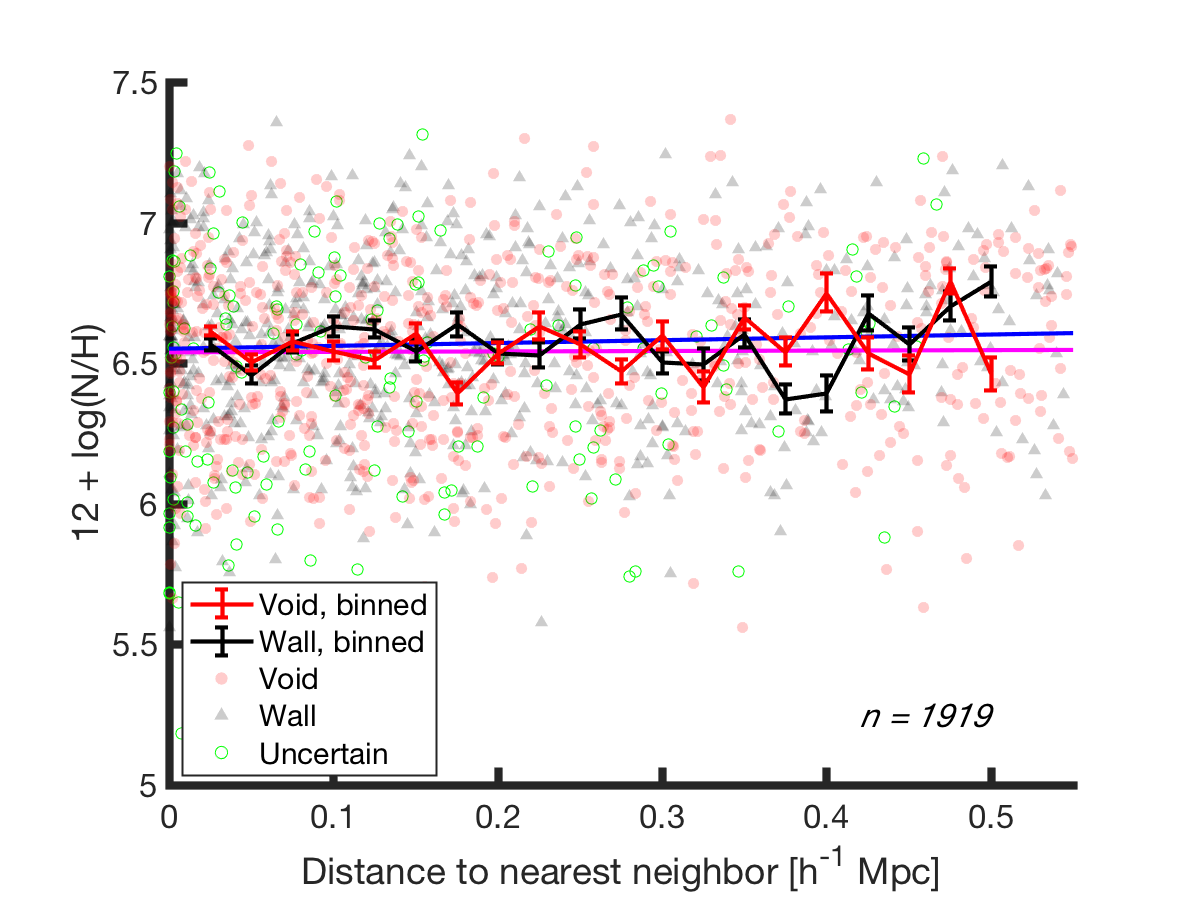
\includegraphics[width=0.49\textwidth]{Images/smallScaleEnvironment/1sig_dwarf_I06relations_absDist_NH}
    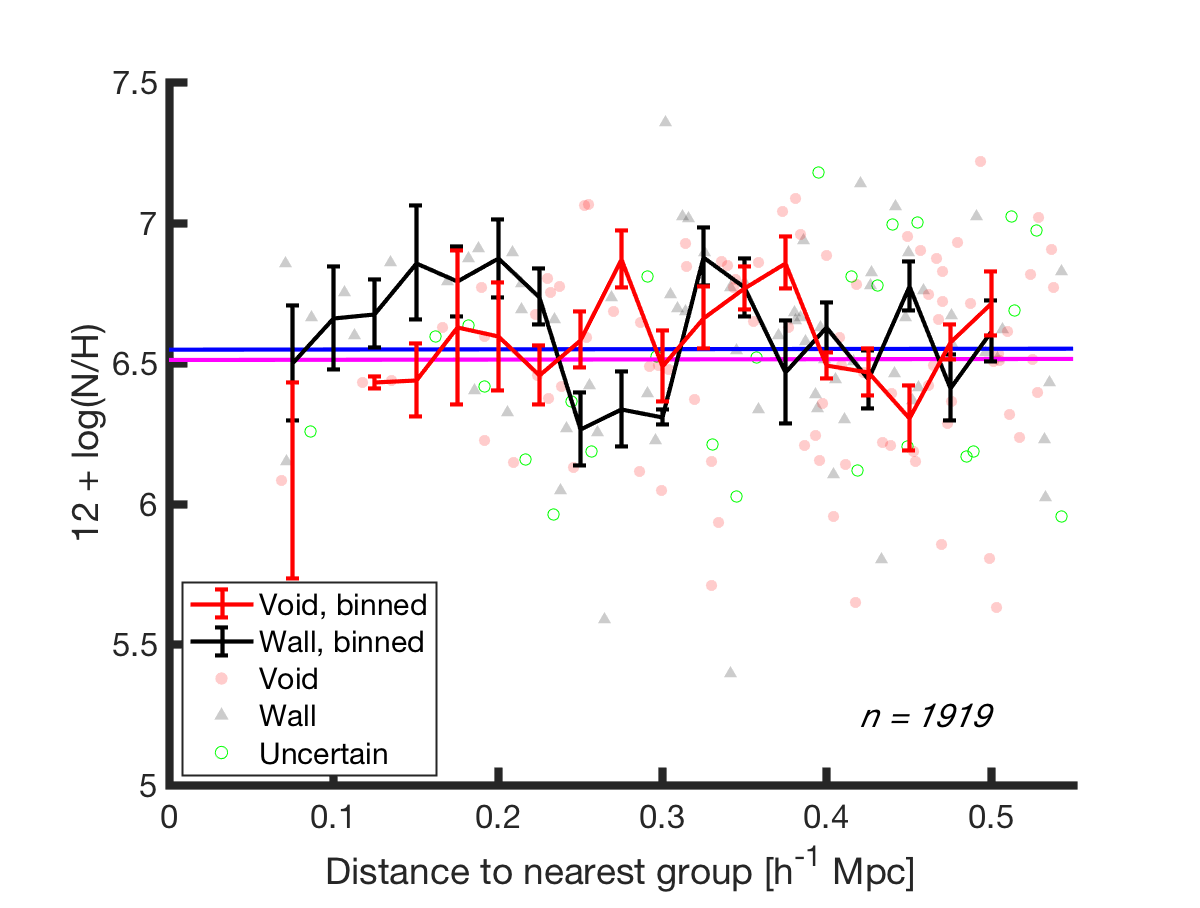
\includegraphics[width=0.49\textwidth]{Images/smallScaleEnvironment/1sig_dwarf_I06relations_groupAbsDist_NH}
    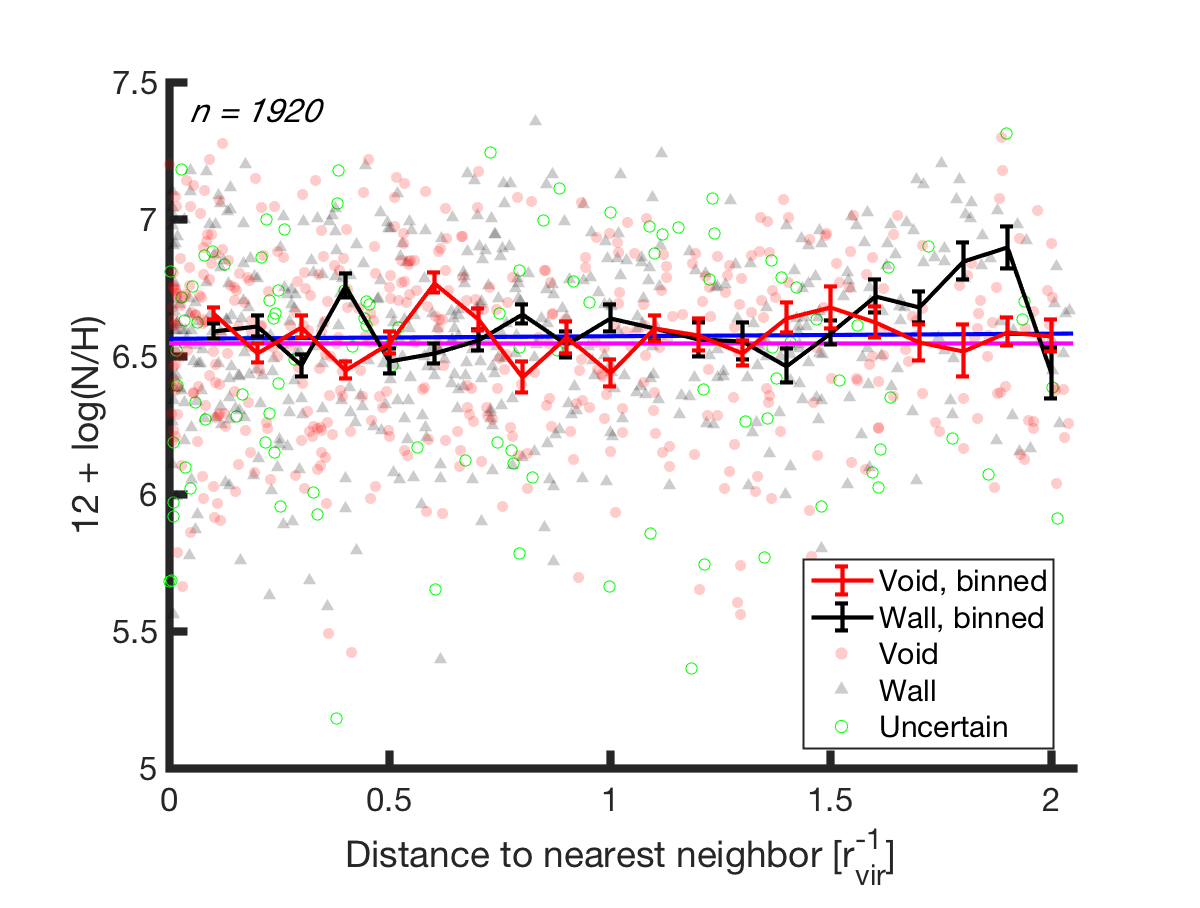
\includegraphics[width=0.49\textwidth]{Images/smallScaleEnvironment/1sig_dwarf_I06relations_virDist_NH}
    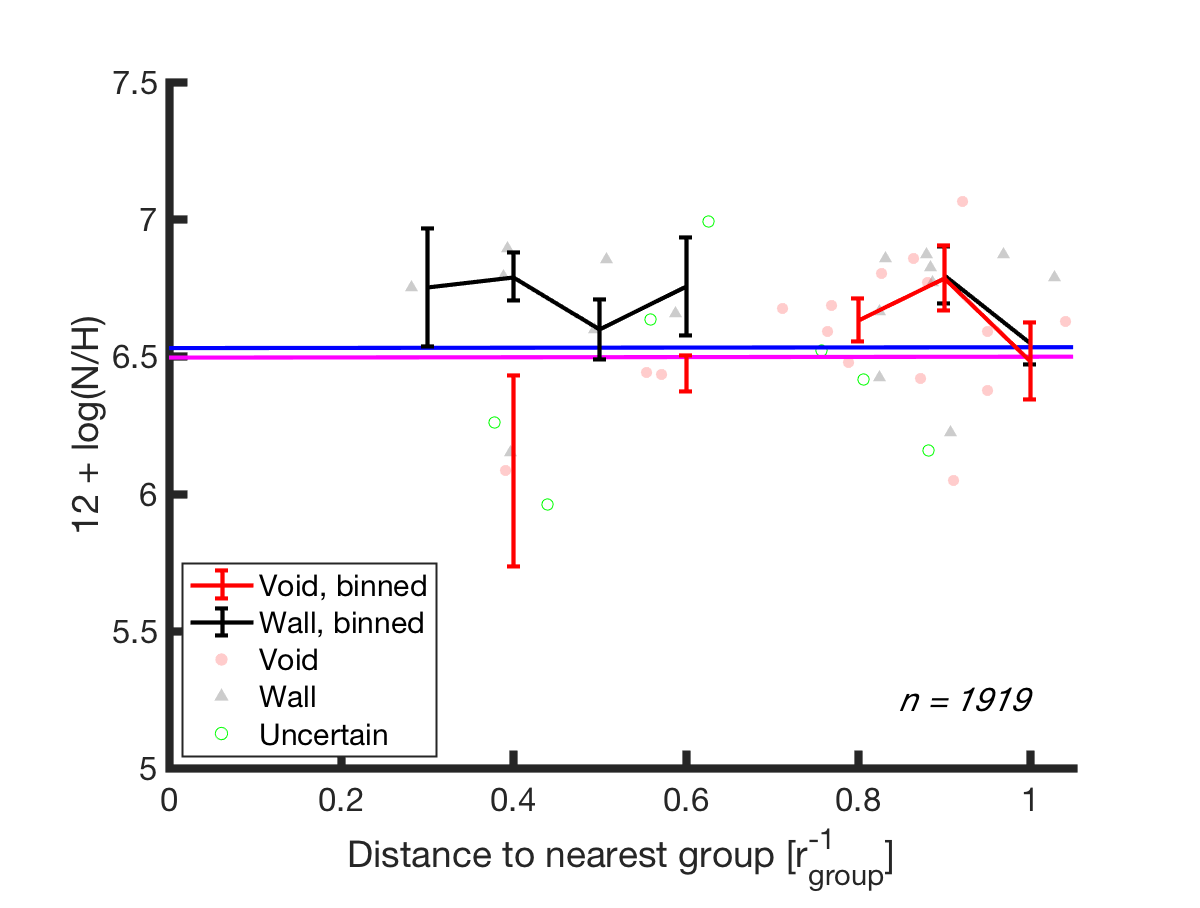
\includegraphics[width=0.49\textwidth]{Images/smallScaleEnvironment/1sig_dwarf_I06relations_groupRDist_NH}
%    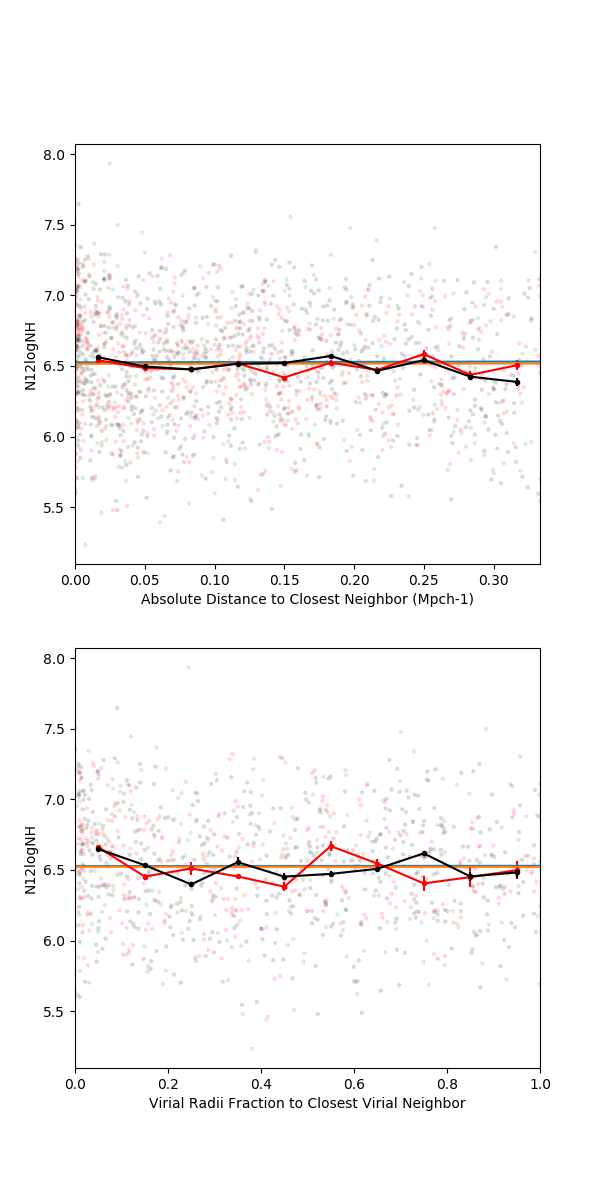
\includegraphics[width=0.49\textwidth]{Images/smallScaleEnvironment/dwarf_NH_300}
%    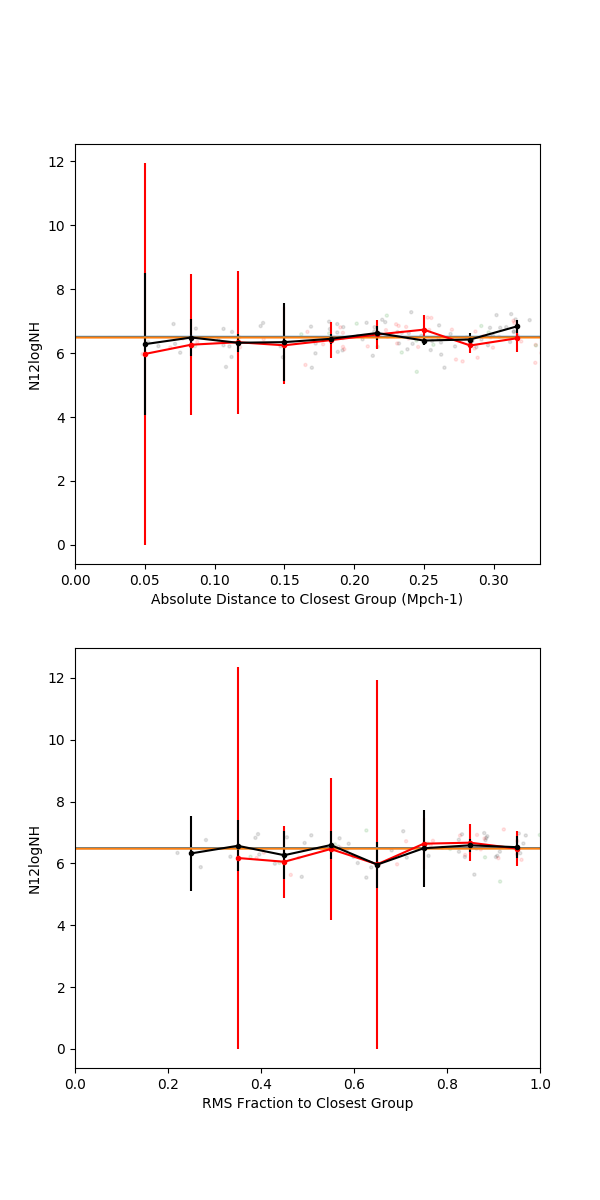
\includegraphics[width=0.49\textwidth]{Images/smallScaleEnvironment/dwarf_NH_300_group}
    \caption[N/H versus distance to nearest neighbor and group]{Gas-phase 
    nitrogen abundance versus distance to the nearest galaxy (on the left) and 
    nearest group (on the right).  The top panels show N/H as a function of the 
    sky separation in \hMpc between the target dwarf galaxy and the neighbor, 
    while the bottom panels show N/H as a function of the closest virial 
    neighbor.  Void galaxies are shown in red, while wall galaxies are shown in 
    black and unknown in green.  We have also included the median nitrogen 
    abundance for the galaxies after binning by distance, to discern any finer 
    behavior in the relationships.  Linear fits to the void and wall galaxies 
    are shown in orange and blue, respectively.  Void dwarf galaxies have 
    slightly lower N/H ratios than dwarf galaxies in denser environments.  
    Otherwise, there does not appear to be any relationship between the dwarf 
    galaxies' nitrogen abundance and the distance to their nearest neighbor.  It 
    appears that void dwarf galaxies within 0.05 \hMpc of a group have slightly 
    lower nitrogen abundances.}
    \label{fig:NH}
\end{figure}

It was expected that the gas-phase nitrogen abundance would follow the same 
trend as the metallicity, to decrease with increasing distance.  As observed 
with the other parameters, Fig. \ref{fig:NH} shows very little relationship 
between the distance and N/H.  The linear fits quantify this observation --- the 
slopes are on the order of 10$^{-3}$, except for the wall dwarf galaxies when 
the distance to the nearest neighbor is measured in \hMpc.  Here, wall dwarf 
galaxies exhibit an increase in the N/H ratio with increasing distance to the 
nearest neighbor.  Within a distance of 0.05 \hMpc of the nearest group, void 
dwarf galaxies tend to have lower nitrogen abundances.  There does not seem to 
be any relationship between the nitrogen abundance of the star-forming dwarf 
galaxies and distance to the nearest galaxy.  We see a slight difference in the 
nitrogen abundance resulting from the large-scale environment, similar to what 
is observed in \cite{Douglass17b} and \cite{Douglass17c}.


\subsubsection{N/O ratio}

\begin{figure}
    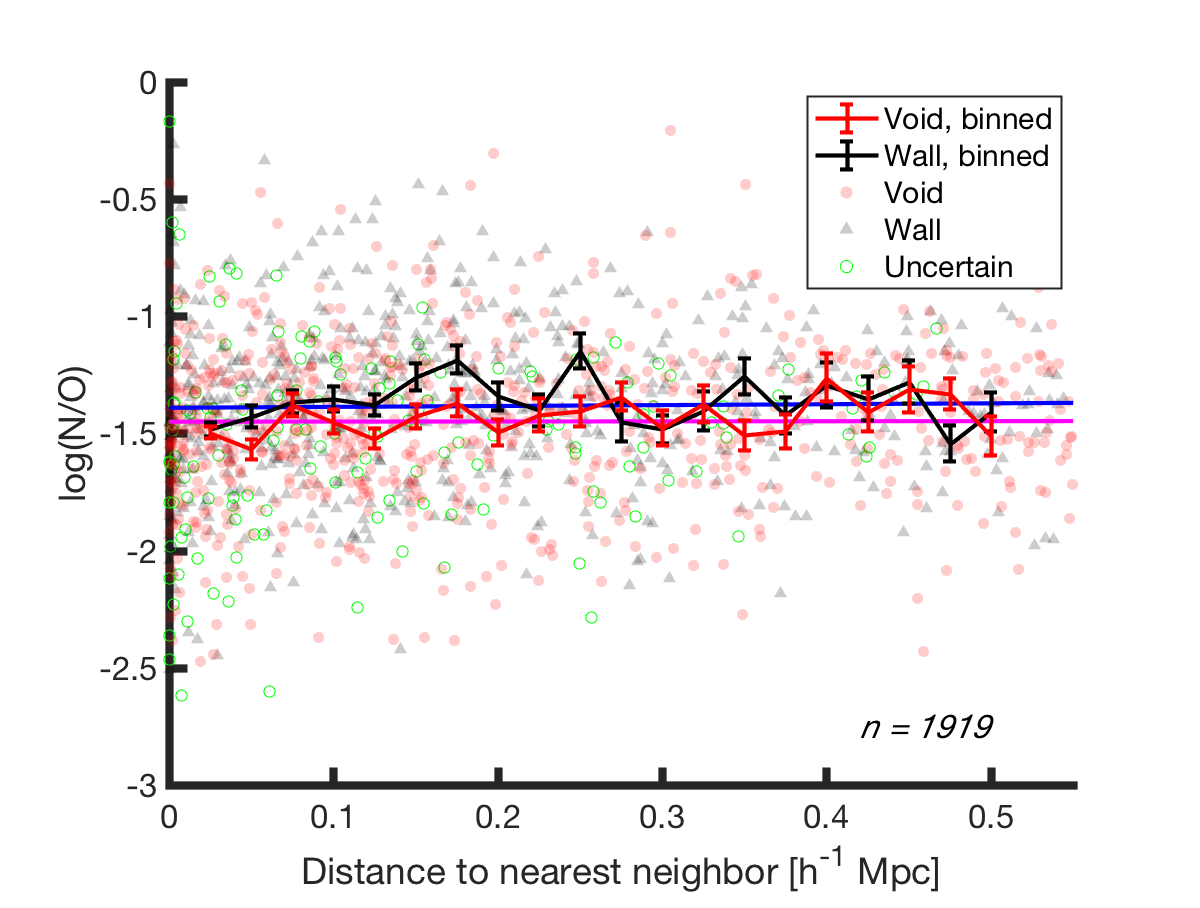
\includegraphics[width=0.49\textwidth]{Images/smallScaleEnvironment/1sig_dwarf_I06relations_absDist_NO}
    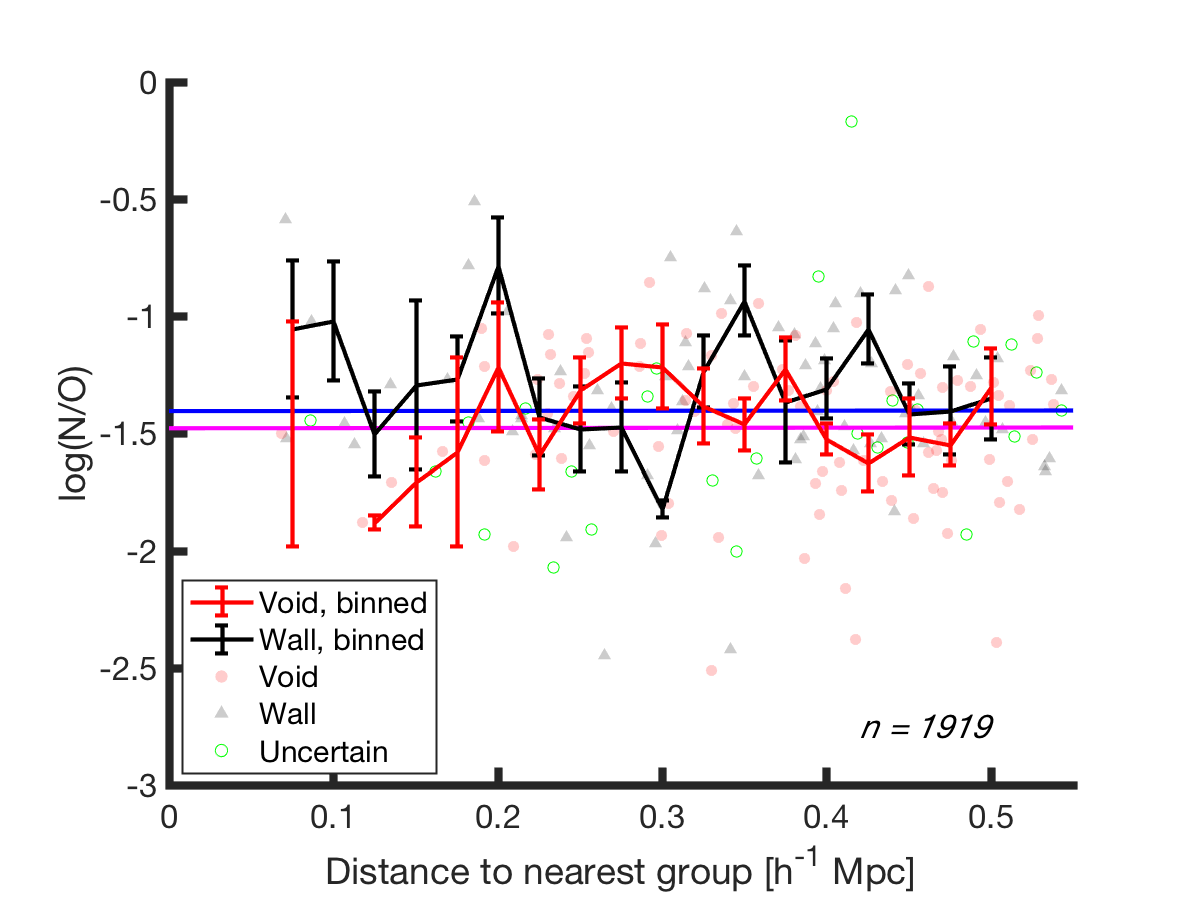
\includegraphics[width=0.49\textwidth]{Images/smallScaleEnvironment/1sig_dwarf_I06relations_groupAbsDist_NO}
    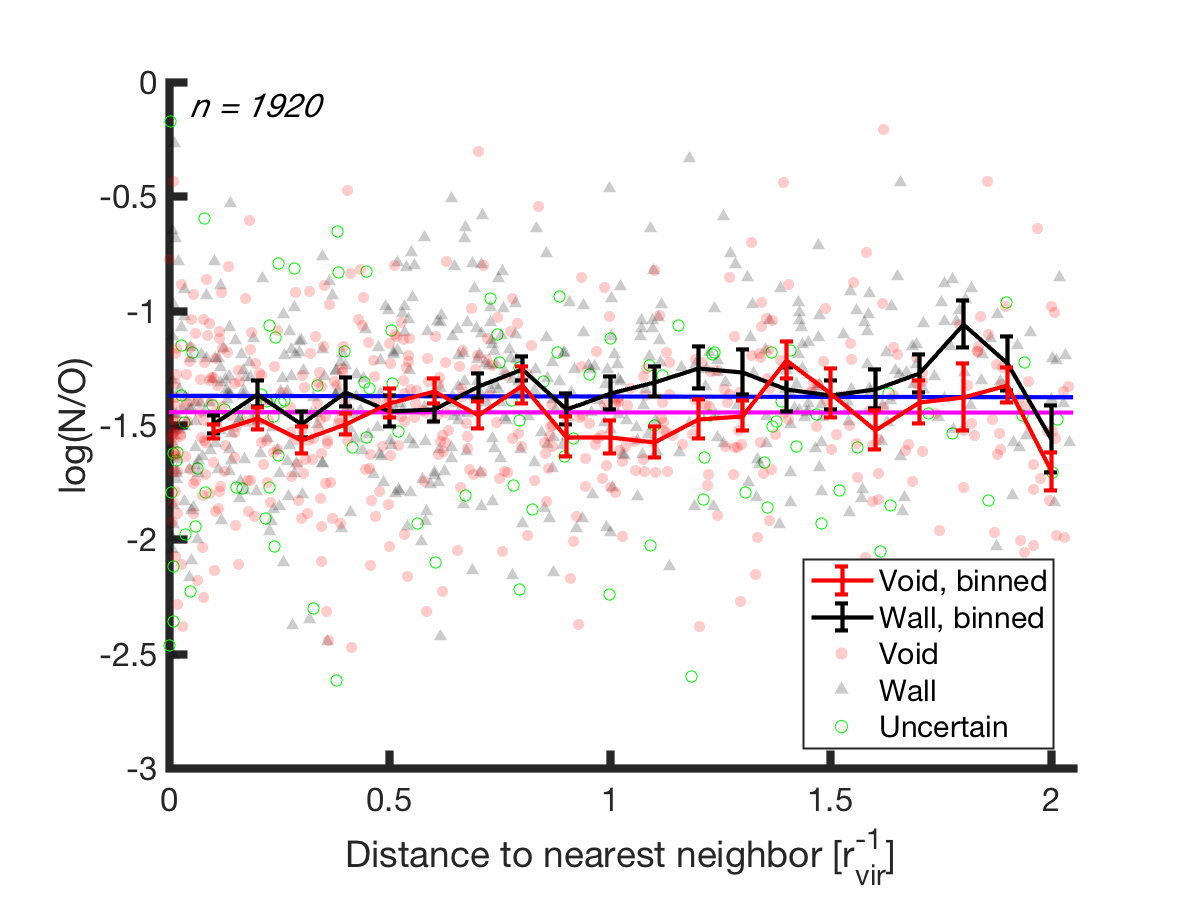
\includegraphics[width=0.49\textwidth]{Images/smallScaleEnvironment/1sig_dwarf_I06relations_virDist_NO}
    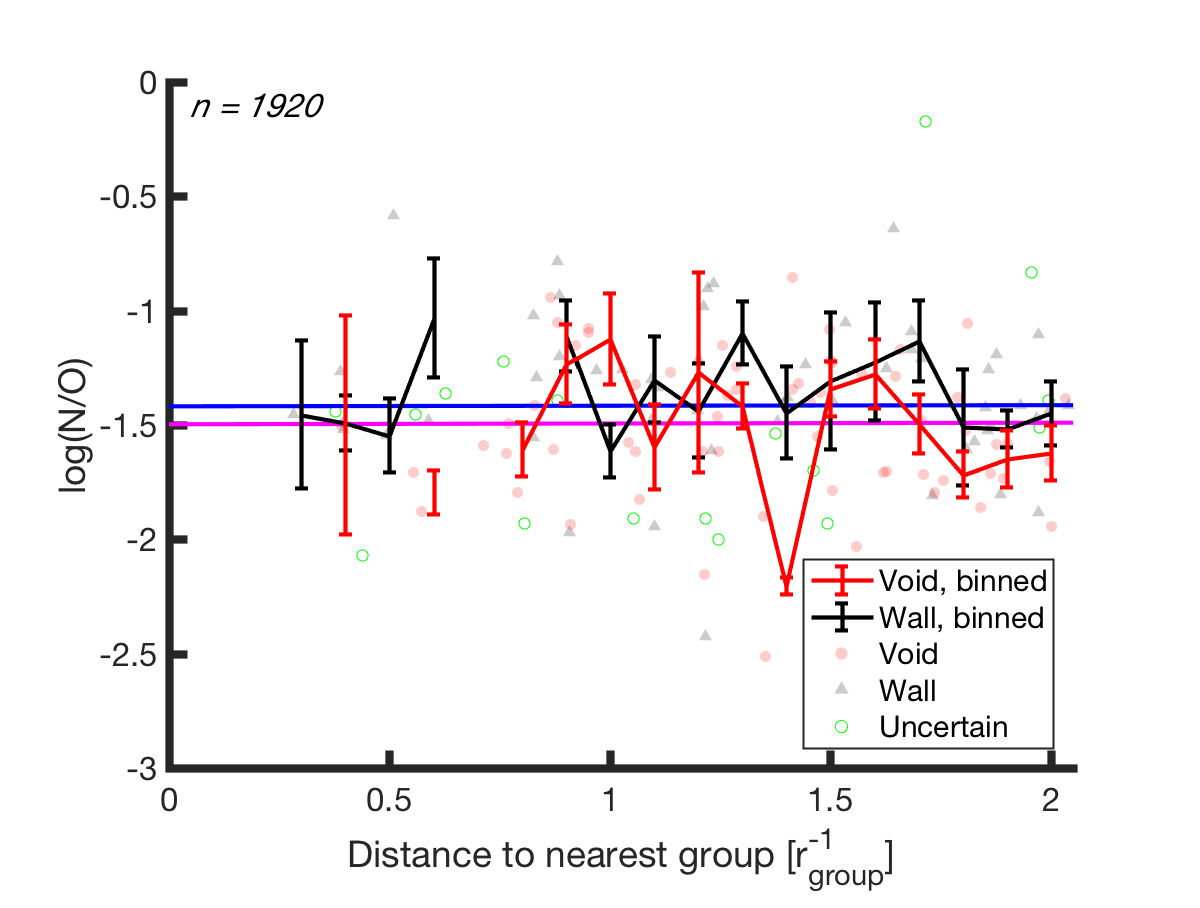
\includegraphics[width=0.49\textwidth]{Images/smallScaleEnvironment/1sig_dwarf_I06relations_groupRDist_NO}
%    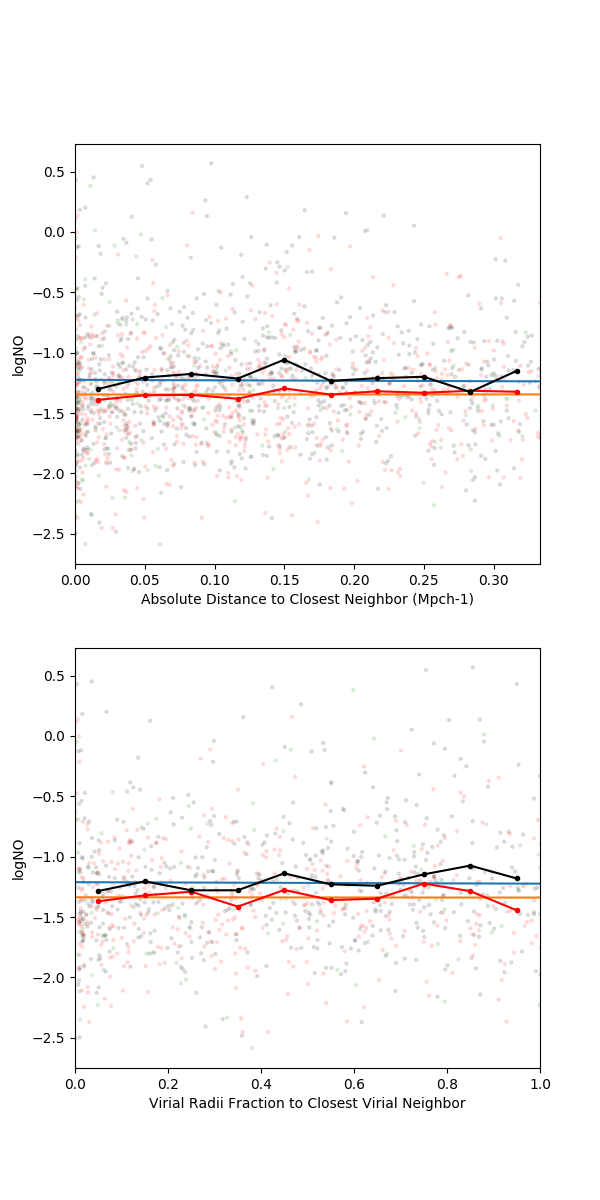
\includegraphics[width=0.49\textwidth]{Images/smallScaleEnvironment/dwarf_NO_300}
%    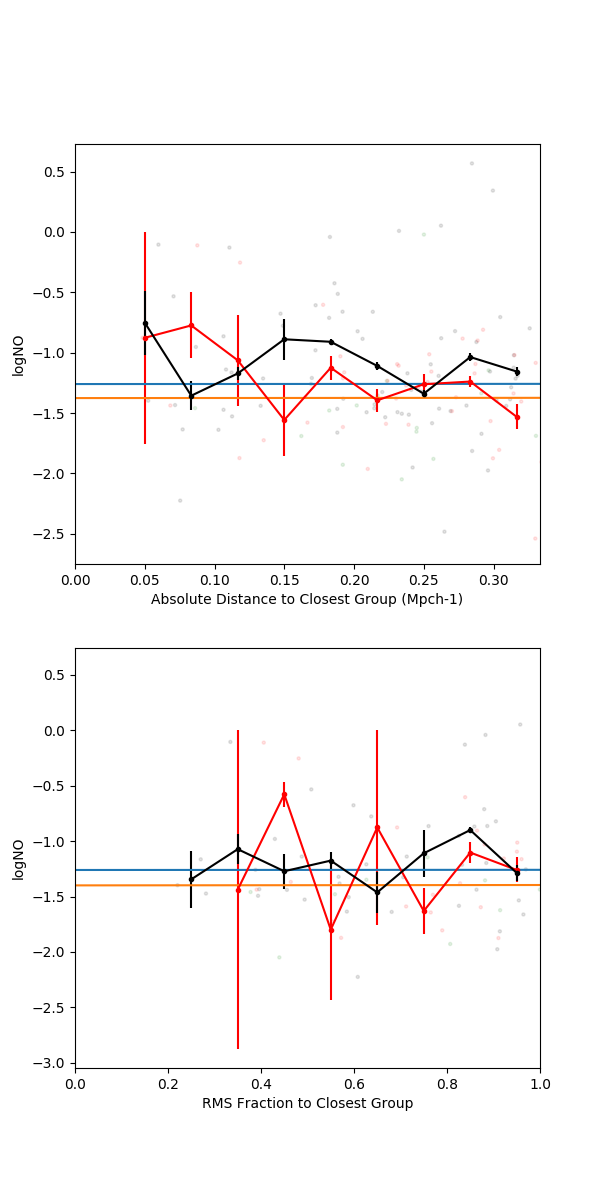
\includegraphics[width=0.49\textwidth]{Images/smallScaleEnvironment/dwarf_NO_300_group}
    \caption[N/O versus distance to nearest neighbor and group]{N/O ratio versus 
    distance to the nearest galaxy (on the left) and nearest group (on the 
    right).  The top panels show the N/O ratio as a function of the sky 
    separation in \hMpc between the target dwarf galaxy and the neighbor, while 
    the bottom panels show N/O as a function of the closest virial neighbor.  
    Void galaxies are shown in red, while wall galaxies are shown in black and 
    unknown in green.  We have also included the median nitrogen abundance for 
    the galaxies after binning by distance, to discern any finer behavior in the 
    relationships.  Linear fits to the void and wall galaxies are shown in 
    orange and blue, respectively.  The void dwarf galaxies have lower N/O 
    ratios than the wall dwarf galaxies.  Within a distance of 0.05 \hMpc from 
    the nearest galaxy, dwarf galaxies appear to have lower N/O ratios.}
    \label{fig:NO}
\end{figure}

Since nucleosynthesis is a physical process unaffected by external influences, 
we do not expect any influence on the relative synthesis of oxygen and nitrogen 
from the proximity to a nearest neighbor.  The upper left plot of Fig. 
\ref{fig:NO} shows that the N/O ratio is lower in dwarf galaxies within 0.05 
\hMpc to a nearest neighbor.  The lack of any other correlation is reflected in 
the linear fits to the data --- the slopes are on the order of 10$^{-3}$.  The 
shift towards lower N/O ratios in star-forming void dwarf galaxies is readily 
apparent, as found by \cite{Douglass17b} and \cite{Douglass17c}.


\subsection{Linear fit parameters}

\begin{table}
    \begin{tabular}{lcccc}
        Property & Slope (void) & Slope (wall) & Intercept (void) & Intercept (wall)\\
        \hline
        \hline
        \multicolumn{5}{c}{Nearest galaxy by distance}\\
        \hline
        $u-r$ & $-0.02\pm 0.027$ & $0.02\pm 0.063$ & $1.05\pm 0.024$  & $1.06\pm 0.031$\\
        sSFR  & $0.01\pm 0.042$  & $0.0\pm 0.10$   & $-9.28\pm 0.037$ & $-9.33\pm 0.049$\\
        \OH   & $0.01\pm 0.027$  & $0.06\pm 0.062$ & $7.99\pm 0.024$  & $7.94\pm 0.030$\\
        \NH   & $0.02\pm 0.028$  & $0.10\pm 0.059$ & $6.54\pm 0.026$  & $6.55\pm 0.029$\\
        \NO   & $0.00\pm 0.028$  & $0.04\pm 0.062$ & $-1.45\pm 0.026$ & $-1.39\pm 0.030$\\
        \hline
        \multicolumn{5}{c}{Nearest galaxy by fraction of virial radius}\\
        \hline
        $u-r$ & $-0.001\pm 0.0043$ & $-0.004\pm 0.0099$ & $1.05\pm 0.026$  & $1.08\pm 0.031$\\
        sSFR  & $0.000\pm 0.0066$  & $0.00\pm 0.016$    & $-9.28\pm 0.040$ & $-9.34\pm 0.049$\\
        \OH   & $0.001\pm 0.0042$  & $0.012\pm 0.0099$  & $7.99\pm 0.025$  & $7.94\pm 0.031$\\
        \NH   & $0.000\pm 0.0045$  & $0.009\pm 0.0094$  & $6.55\pm 0.027$  & $6.56\pm 0.029$\\
        \NO   & $-0.001\pm 0.0045$ & $-0.003\pm 0.0098$ & $-1.44\pm 0.027$ & $-1.37\pm 0.031$\\
        \hline
        \multicolumn{5}{c}{Nearest group by distance}\\
        \hline
        $u-r$ & $0.002\pm 0.0042$  & $-0.002\pm 0.0041$ & $1.03\pm 0.029$  & $1.08\pm 0.033$\\
        sSFR  & $-0.003\pm 0.0064$ & $0.006\pm 0.0065$  & $-9.26\pm 0.045$ & $-9.36\pm 0.053$\\
        \OH   & $0.001\pm 0.0041$  & $0.002\pm 0.0041$  & $7.99\pm 0.029$  & $7.95\pm 0.033$\\
        \NH   & $0.007\pm 0.0043$  & $0.006\pm 0.0038$  & $6.51\pm 0.031$  & $6.55\pm 0.031$\\
        \NO   & $0.006\pm 0.0044$  & $0.005\pm 0.0040$  & $-1.48\pm 0.031$ & $-1.40\pm 0.033$\\
        \hline
        \multicolumn{5}{c}{Nearest group by fraction of group radius}\\
        \hline
        $u-r$ & $0.001\pm 0.0018$  & $-0.001\pm 0.0017$ & $1.02\pm 0.033$  & $1.08\pm 0.036$\\
        sSFR  & $-0.002\pm 0.0027$ & $0.002\pm 0.0028$  & $-9.24\pm 0.051$ & $-9.37\pm 0.058$\\
        \OH   & $0.000\pm 0.0017$  & $0.001\pm 0.0017$  & $7.99\pm 0.033$  & $7.95\pm 0.036$\\
        \NH   & $0.003\pm 0.0018$  & $0.004\pm 0.0016$  & $6.50\pm 0.034$  & $6.53\pm 0.034$\\
        \NO   & $0.003\pm 0.0018$  & $0.002\pm 0.0017$  & $-1.50\pm 0.034$ & $-1.42\pm 0.036$
    \end{tabular}
    \caption[Fit parameters of properties versus distances]{Linear fit 
    parameters to various properties of the target dwarf galaxies by their 
    distances to the nearest galaxy in units of \hMpc, the nearest galaxy in 
    units of the neighbor's virial radius, the center of the nearest group in 
    units of \hMpc, and the nearest group in units of the group's rms radius; 
    all objects must be within 300 km/s of the target galaxy.  Except for the 
    relationship between the nitrogen abundance of wall dwarf galaxies and the 
    distance to the nearest neighbor in units of \hMpc, the slopes are all 
    negligible.  This quantifies the observations made that the proximity to a 
    galaxy or group has little influence on a dwarf galaxy's evolution.}
    \label{tab:fits}
\end{table}

To quantify the results shown in Figs. \ref{fig:ur}--\ref{fig:NO}, we calculate 
the parameters for the best linear fit for each physical parameter and distance 
metric combination.  Any slope of significant magnitude shows an overall 
correlation between a given physical parameter and the galaxy's distance to its 
nearest neighbor or group.  The results of this analysis are listed in Table 
\ref{tab:fits}.  These slopes reflect the observations described in Section 
\ref{sec:Relations}: there is no correlation between the distance to the nearest 
neighbor and a galaxy's color, sSFR, or gas-phase chemical abundances, except 
for wall dwarf galaxies and their nitrogen abundances when compared to the 
distance to the nearest galaxy in \hMpc.  This analysis does not capture any 
small variations within the range of distances for all dwarf galaxies included 
in this study.


\subsection{Selection effects}\label{sec:selection_effects}

% Peculiar velocity
\begin{figure}
    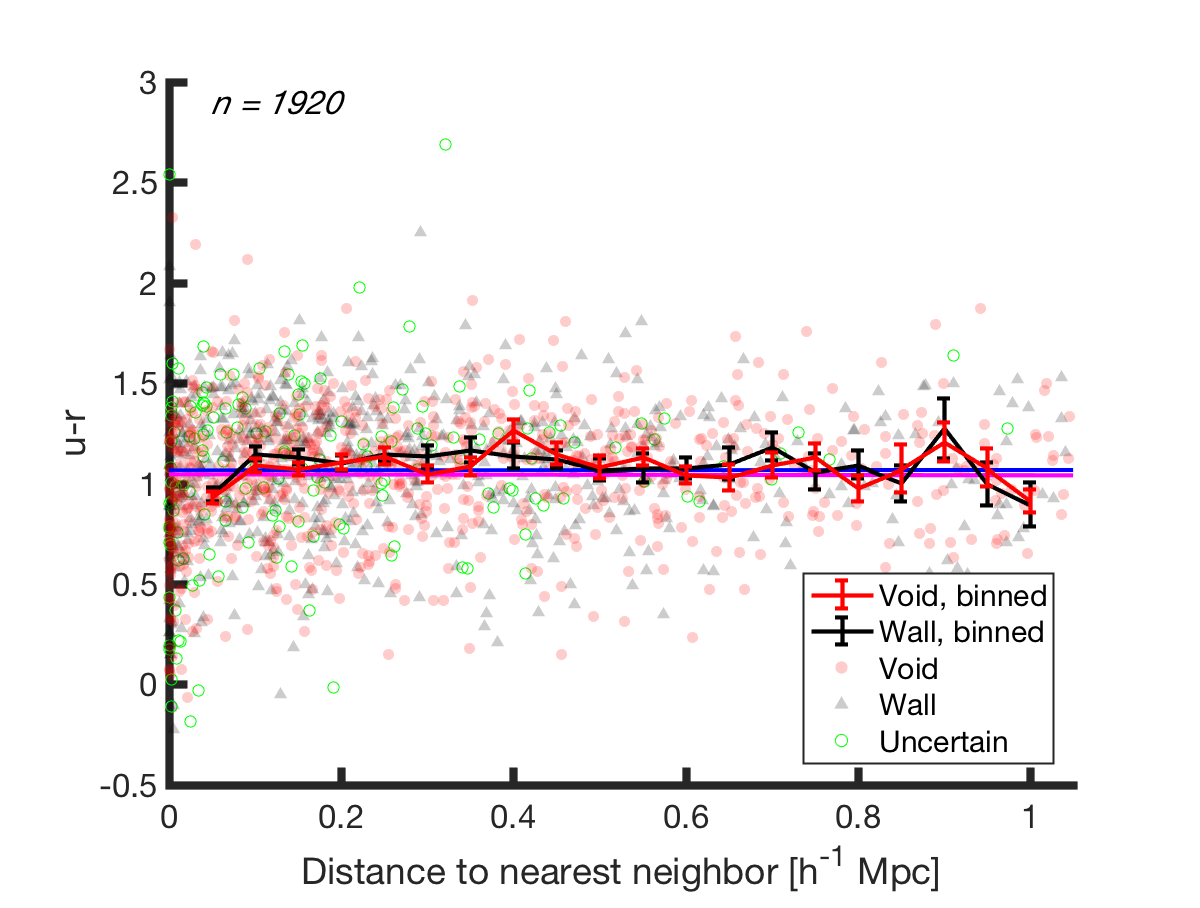
\includegraphics[width=0.49\textwidth]{Images/smallScaleEnvironment/1sig_dwarf_I06relations_absDist150_ur}
    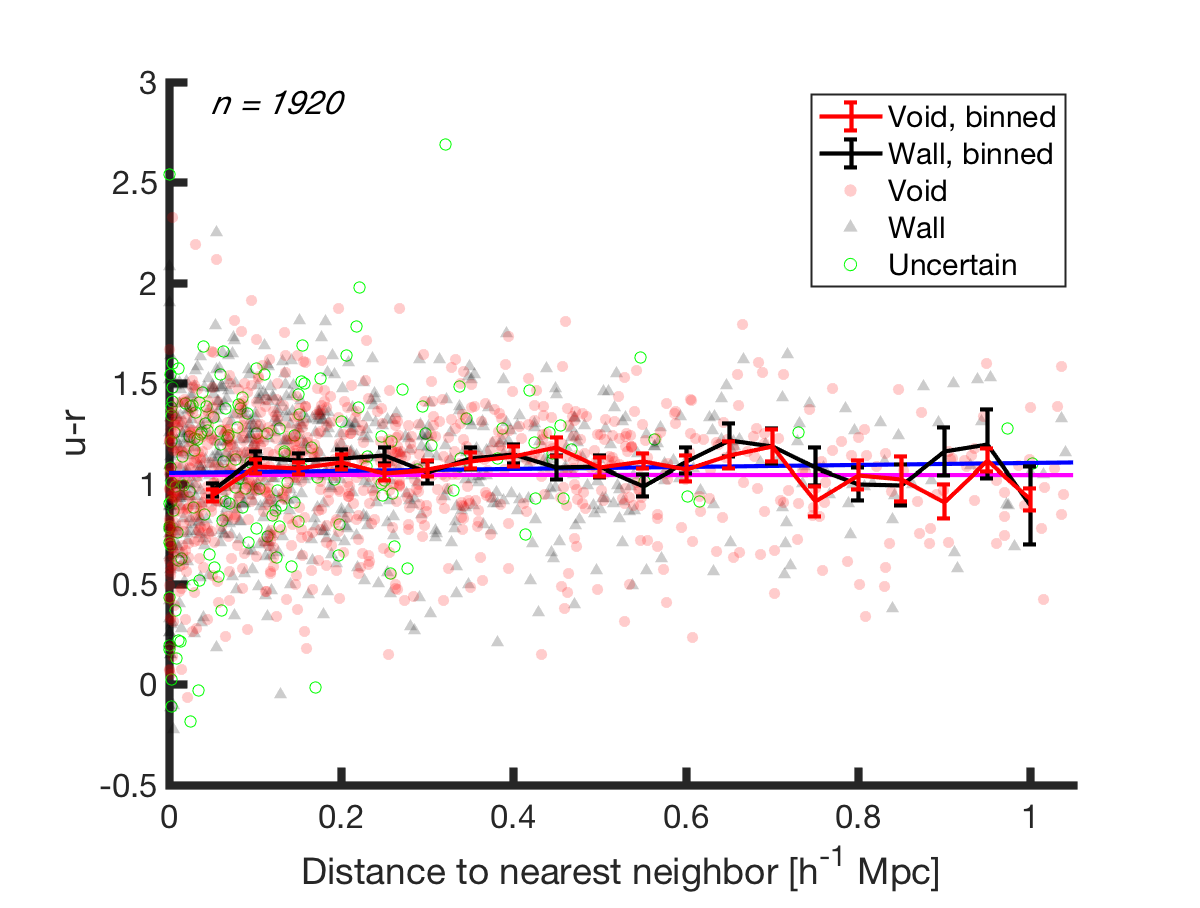
\includegraphics[width=0.49\textwidth]{Images/smallScaleEnvironment/1sig_dwarf_I06relations_absDist600_ur}
    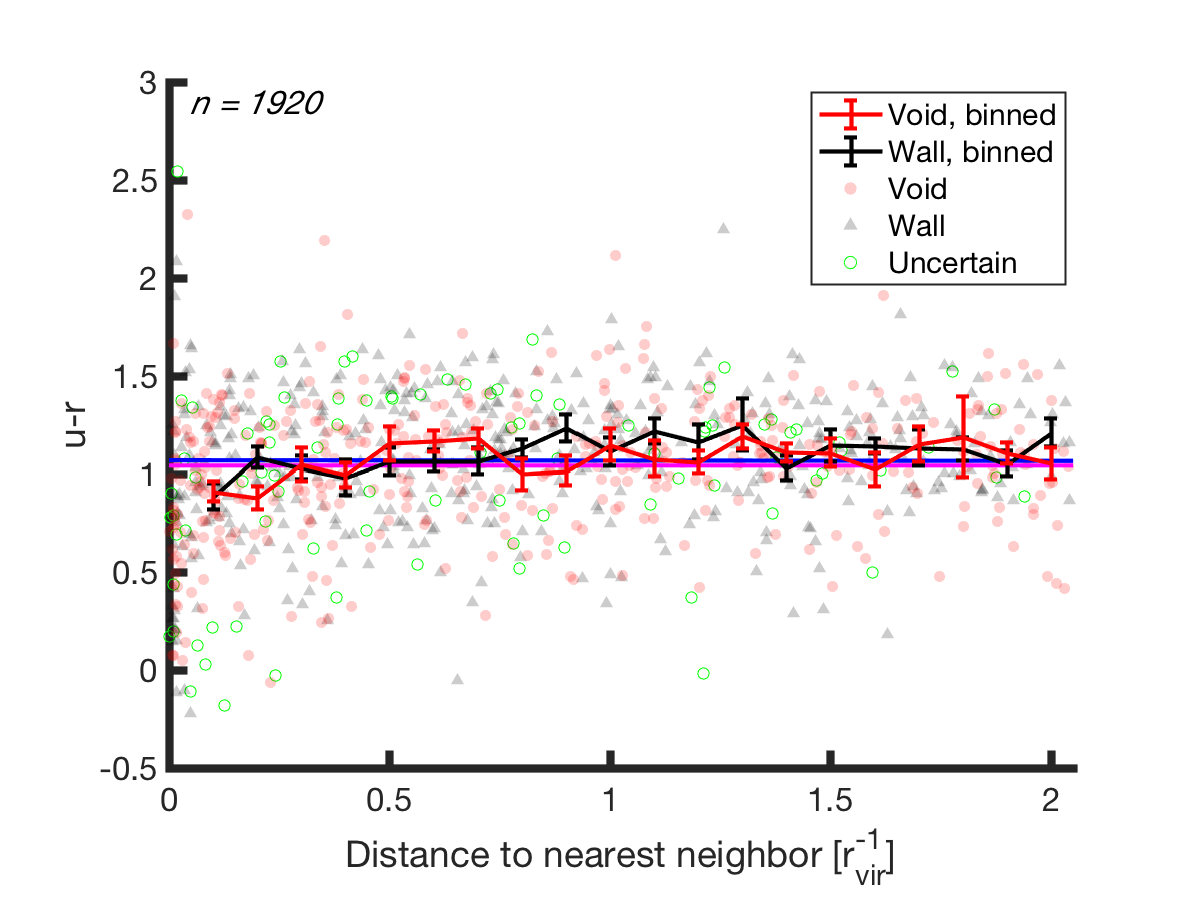
\includegraphics[width=0.49\textwidth]{Images/smallScaleEnvironment/1sig_dwarf_I06relations_virDist150_ur}
    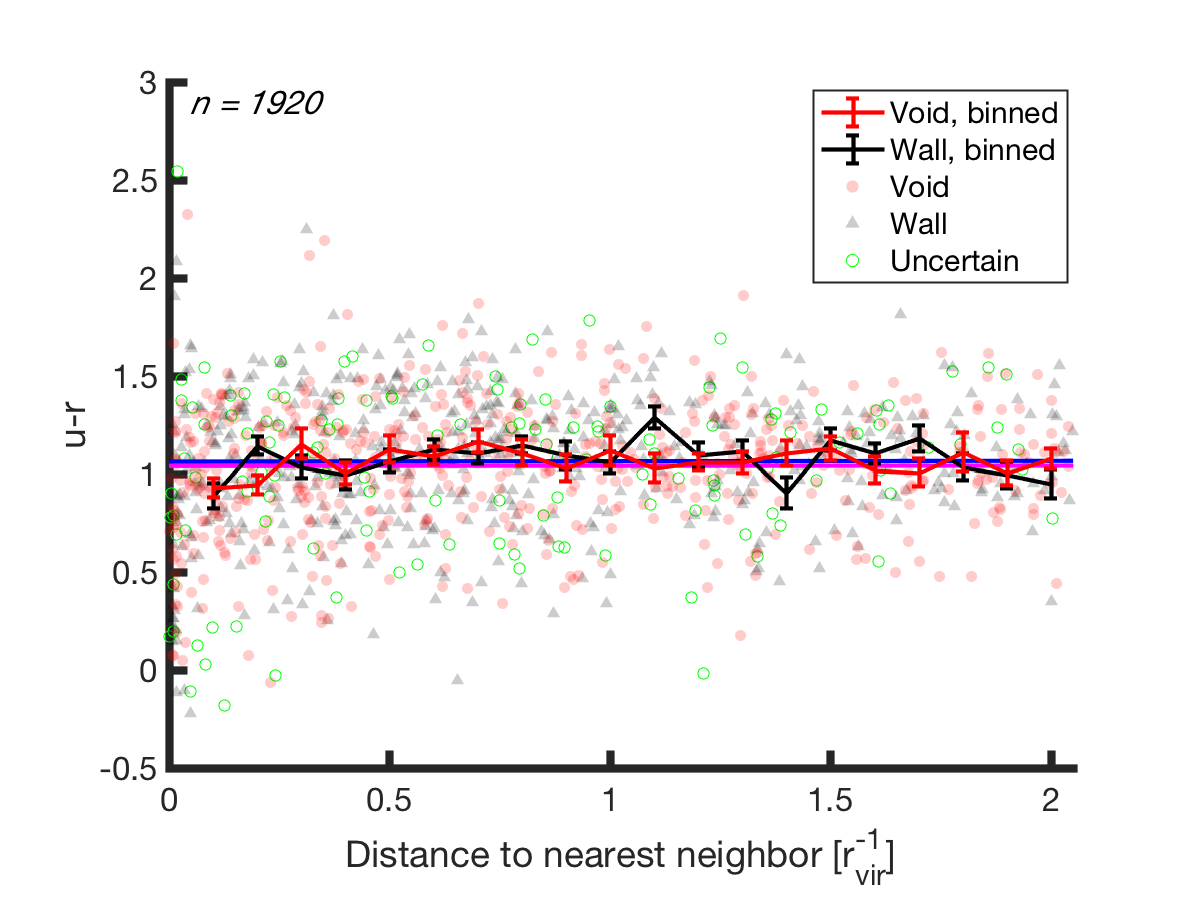
\includegraphics[width=0.49\textwidth]{Images/smallScaleEnvironment/1sig_dwarf_I06relations_virDist600_ur}
%    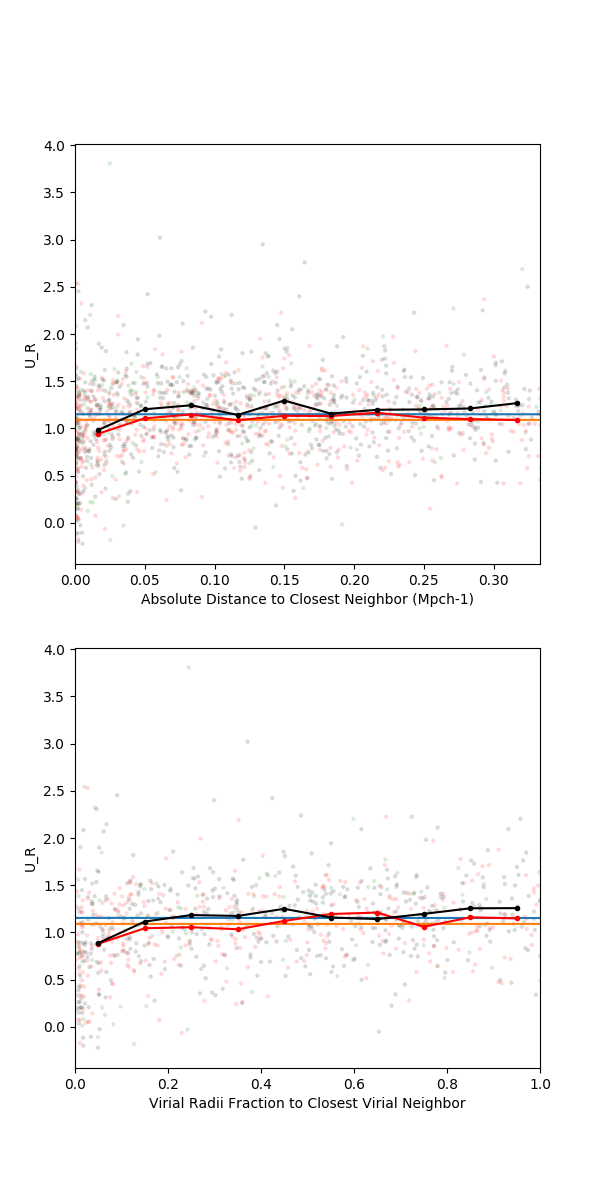
\includegraphics[width=0.49\textwidth]{Images/smallScaleEnvironment/dwarf_ur_150}
%    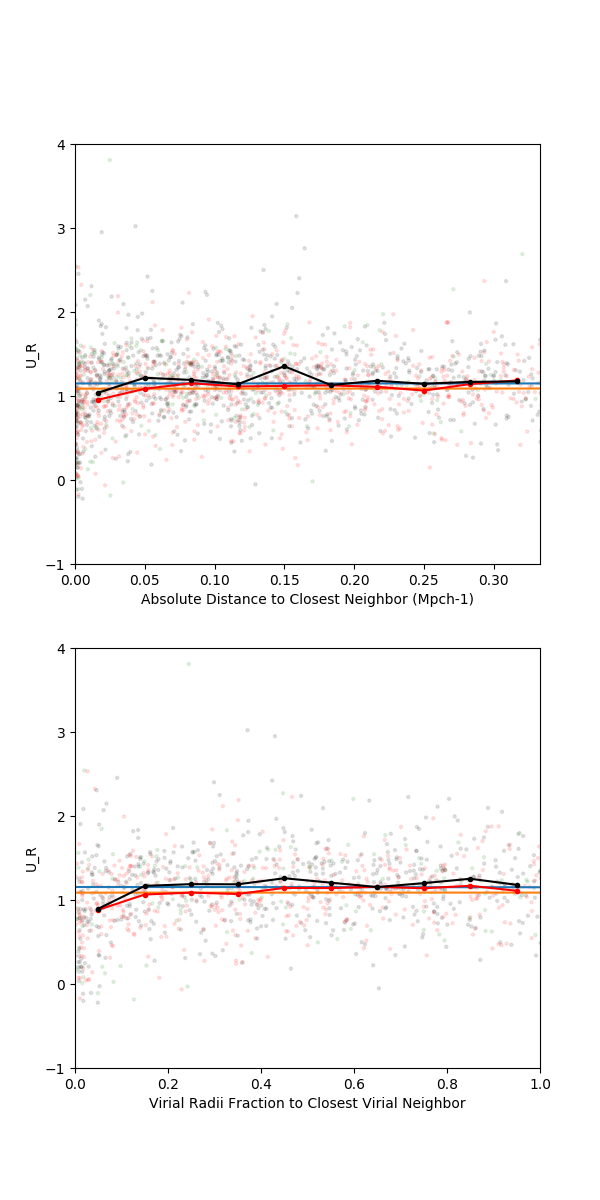
\includegraphics[width=0.49\textwidth]{Images/smallScaleEnvironment/dwarf_ur_600}
    \caption[Sensitivity to peculiar velocity maximum]{Color versus distance to 
    nearest galaxy (in units of \hMpc on top and virial radii on bottom), with a 
    maximum allowed peculiar velocity of 150 km/s in the left panel and 600 km/s 
    in the right panel.  Void galaxies are shown in red, wall in black, and 
    unknown in green.  The galaxies are binned by distance to tease out any 
    trends at smaller distance scales; linear fits to the void and wall galaxies 
    are shown in orange and blue, respectively.  When compared with the two 
    plots in the left panel of Fig. \ref{fig:ur}, we see that there is no 
    significant influence on our results from the choice of maximum peculiar 
    velocity allowed.}
    \label{fig:ur_vpeculiar}
\end{figure}

We test two components of our nearest neighbor criteria to understand how 
sensitive our results are to any initial conditions.  The first parameter we 
discuss is the sensitivity of our results on the maximum peculiar velocity used 
to define a match.  Throughout our analysis, we use 300 km/s as the maximum 
velocity separation allowed between the target galaxy and its nearest neighbor 
or group.  We look at how this affects our results by repeating the analysis 
with maximum velocities of 150 km/s and 600 km/s \citep[the criteria used in][]
{Hwang10,Guo11}.  The results of this comparison on the color of the galaxies 
can be seen in Fig. \ref{fig:ur_vpeculiar}.  The nearest neighbors in the 
left-hand panel are restricted to a maximum peculiar velocity of 150 km/s, while 
those in the right panel are restricted to 600 km/s.  When compared to each 
other and to the left-hand panel of Fig. \ref{fig:ur}, it is clear that our 
choice of maximum peculiar velocity has no affect on the results of the study.

% Spectroscopic sample v. complete sample
\begin{figure}
    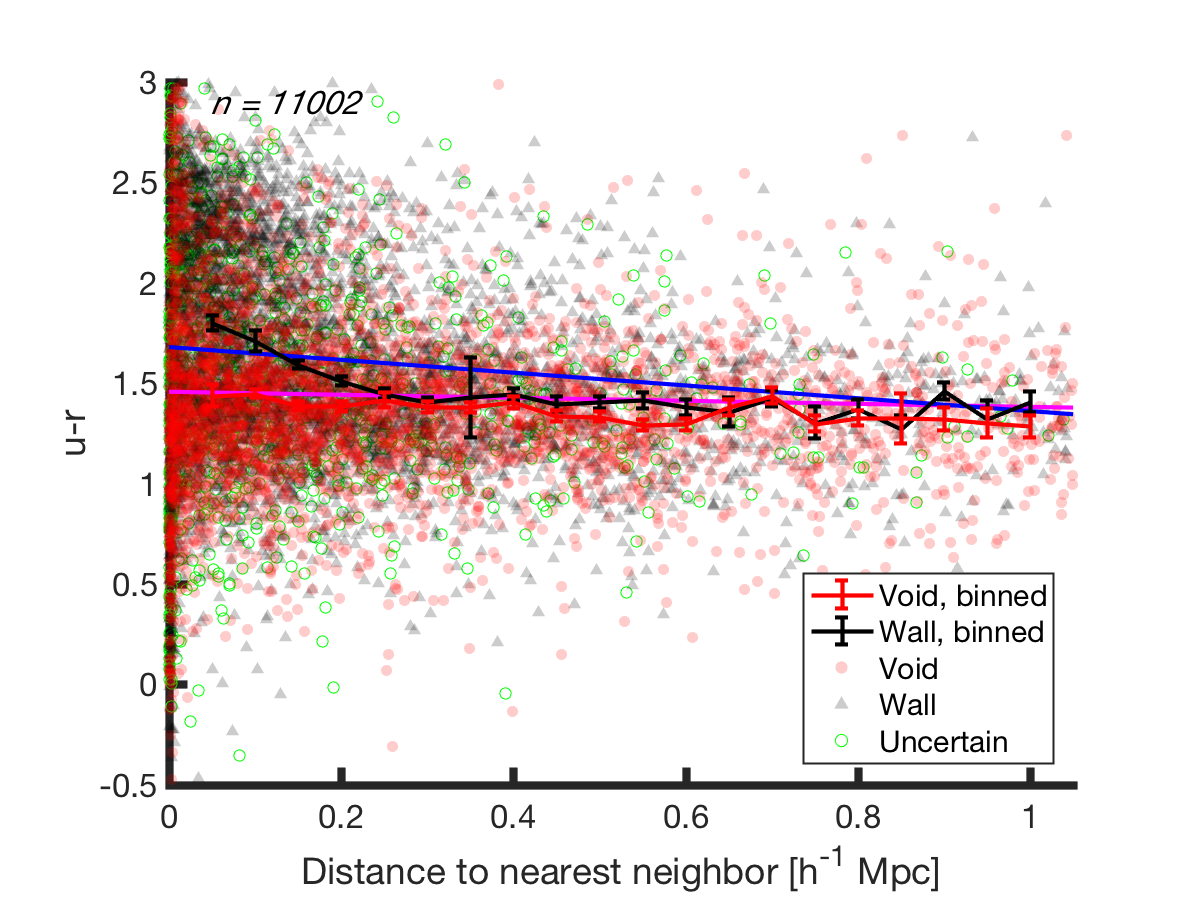
\includegraphics[width=0.49\textwidth]{Images/smallScaleEnvironment/dwarf_absDist_ur}
    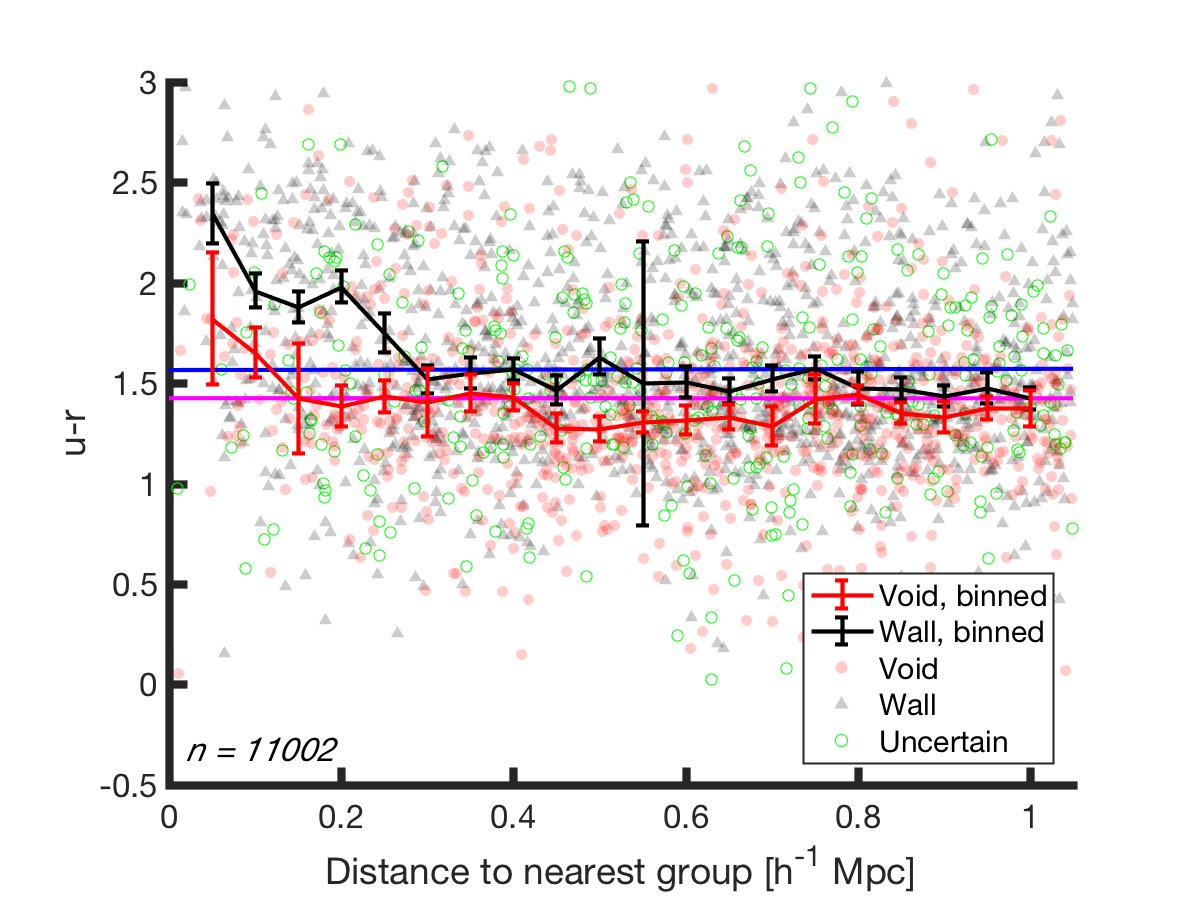
\includegraphics[width=0.49\textwidth]{Images/smallScaleEnvironment/dwarf_groupAbsDist_ur}
    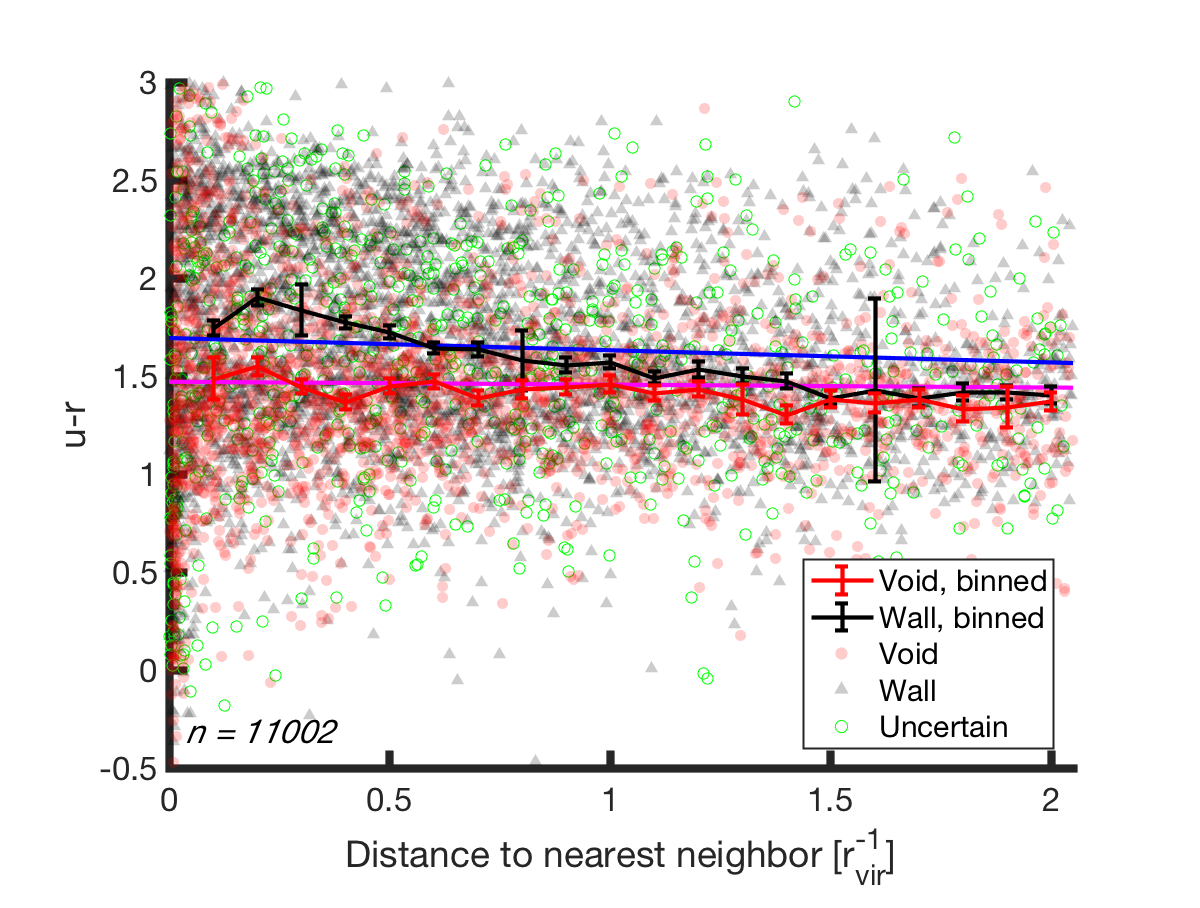
\includegraphics[width=0.49\textwidth]{Images/smallScaleEnvironment/dwarf_virDist_ur}
    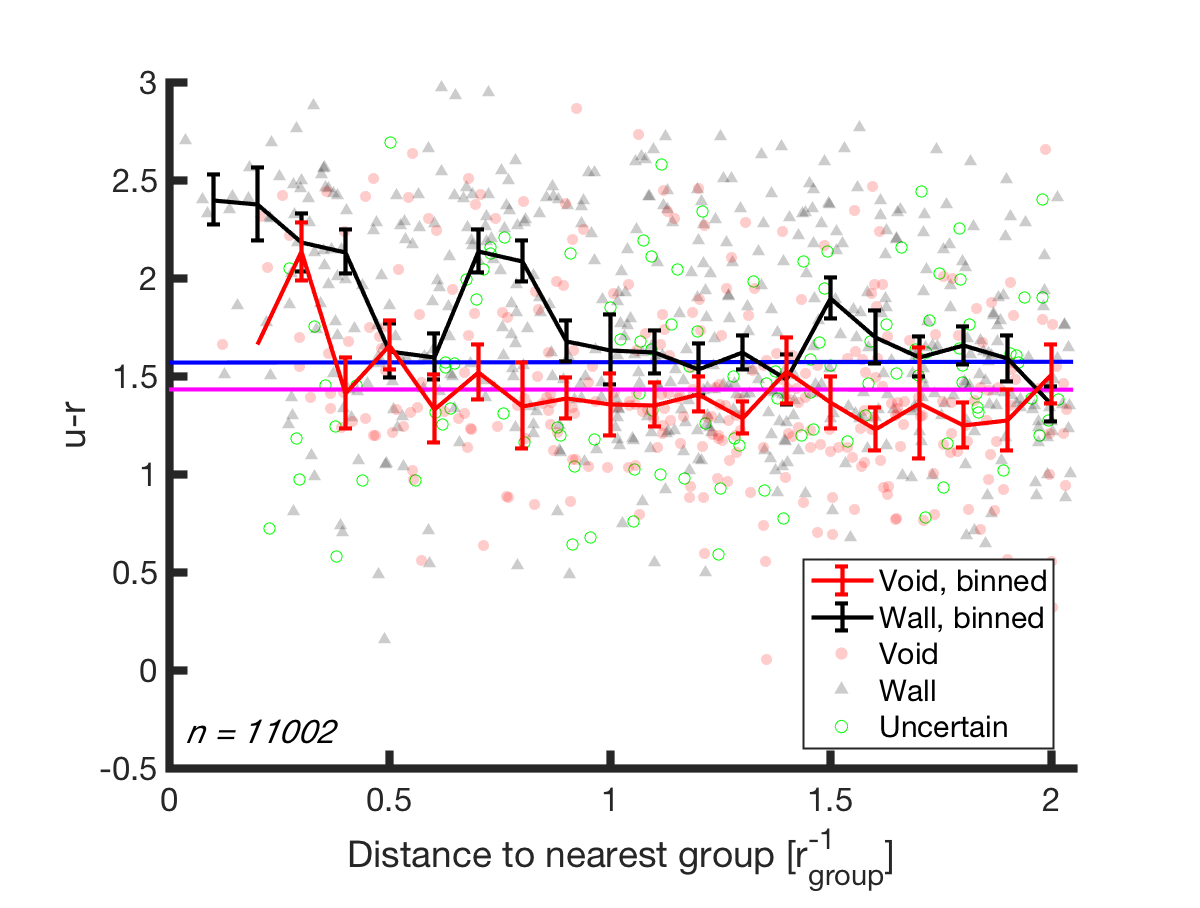
\includegraphics[width=0.49\textwidth]{Images/smallScaleEnvironment/dwarf_groupRDist_ur}
%    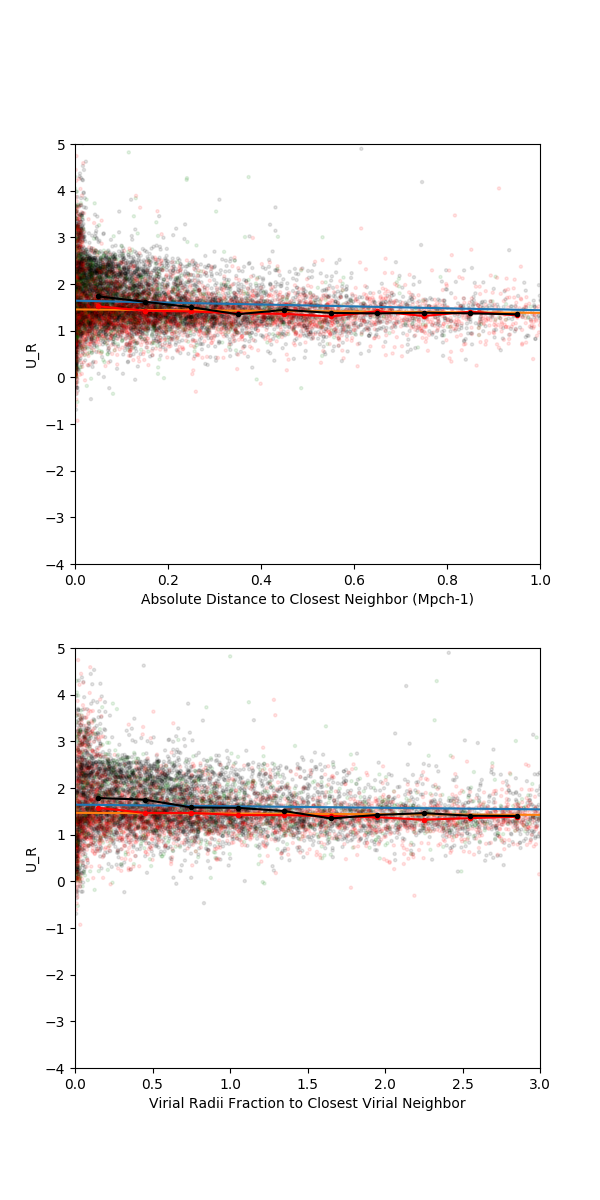
\includegraphics[width=0.5\textwidth]{Images/smallScaleEnvironment/ALLdwarf_ur_300}
    \caption[Color versus distance of full SDSS dwarf population]{Color versus 
    distance to the nearest galaxy (in units of \hMpc on top left and virial 
    radius on the bottom left) and to the center of the nearest group (in units 
    of \hMpc on the top right and group radius on the bottom right) for the 
    entire dwarf galaxy population in SDSS DR7.  When compared to Fig. 
    \ref{fig:ur}, we see that there are some differences in the results of the 
    analysis by studying only star-forming galaxies with sufficient detection of 
    the various emission lines necessary to estimate the gas-phase chemical 
    abundances.  The addition of redder dwarf galaxies to the sample produces an 
    overall inverse relationship between a wall dwarf galaxy's color and the 
    distance to the nearest neighbor in \hMpc and $r_{vir}$.}
    \label{fig:ur_allDwarf}
\end{figure}

We also test the sensitivity of our results to the population of galaxies being 
studied.  Because we want to look at the relationship between distance and the 
gas-phase chemical abundances of the dwarf galaxies, our sample is limited to 
star-forming dwarf galaxies with detected emission lines necessary for 
estimation of the chemical abundances with the Direct $T_e$ method 
\citep[see][for more details]{Douglass17a}.  We perform the same distance 
analysis on all dwarf galaxies detected in SDSS DR7 with respect to their 
color, to understand how our results depend on our sample.  When we compare Fig. 
\ref{fig:ur_allDwarf} with Fig. \ref{fig:ur}, we see that there are some 
differences in the correlation between color and distance to the nearest 
neighbor.  Let us first look at the linear fits to the data.  The upper left 
panel of Fig. \ref{fig:ur_allDwarf} shows that wall dwarf galaxies become redder 
with decreasing distance to their nearest neighbors, while the upper left panel 
of Fig. \ref{fig:ur} shows no such global trend.  In addition, the full dwarf 
galaxy sample also exhibits different behaviors between the void dwarf galaxies 
and the wall dwarf galaxies.  While there is very little relationship between a 
void dwarf galaxy's color and its distance to a nearest neighbor (as seen in 
Fig. \ref{fig:ur}), wall dwarf galaxies are significantly redder than void dwarf 
galaxies within distances of 0.3 \hMpc.

A similar pattern in seen when the distance to the nearest neighbor is measured 
by $r_{vir}$.  Within $r_{vir}$, the bottom left panel of Fig. 
\ref{fig:ur_allDwarf} shows that wall dwarf galaxies are redder than void dwarf 
galaxies.  Within 0.1$r_{vir}$, wall dwarf galaxies are bluer than the global 
trend.  Similar trends are seen in the relationship between color and distance 
to the nearest group, seen in the right panel of Fig. \ref{fig:ur_allDwarf}.  It 
is clear that our selection bias to star-forming dwarf galaxies influences the 
trends we observe for wall dwarf galaxies in our analysis.

% Absolute magnitude distribution of nearest neighbors
\begin{figure}
    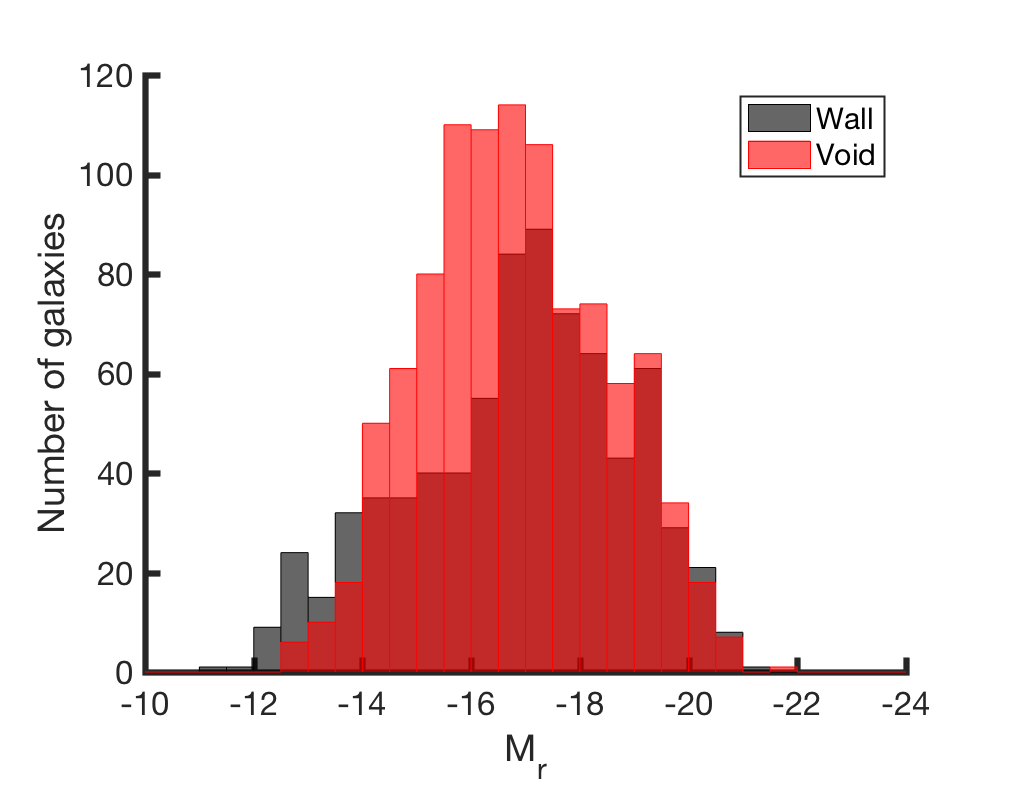
\includegraphics[width=0.49\textwidth]{Images/smallScaleEnvironment/1sig_dwarf_I06relations_rabsmag_abs_hist}
    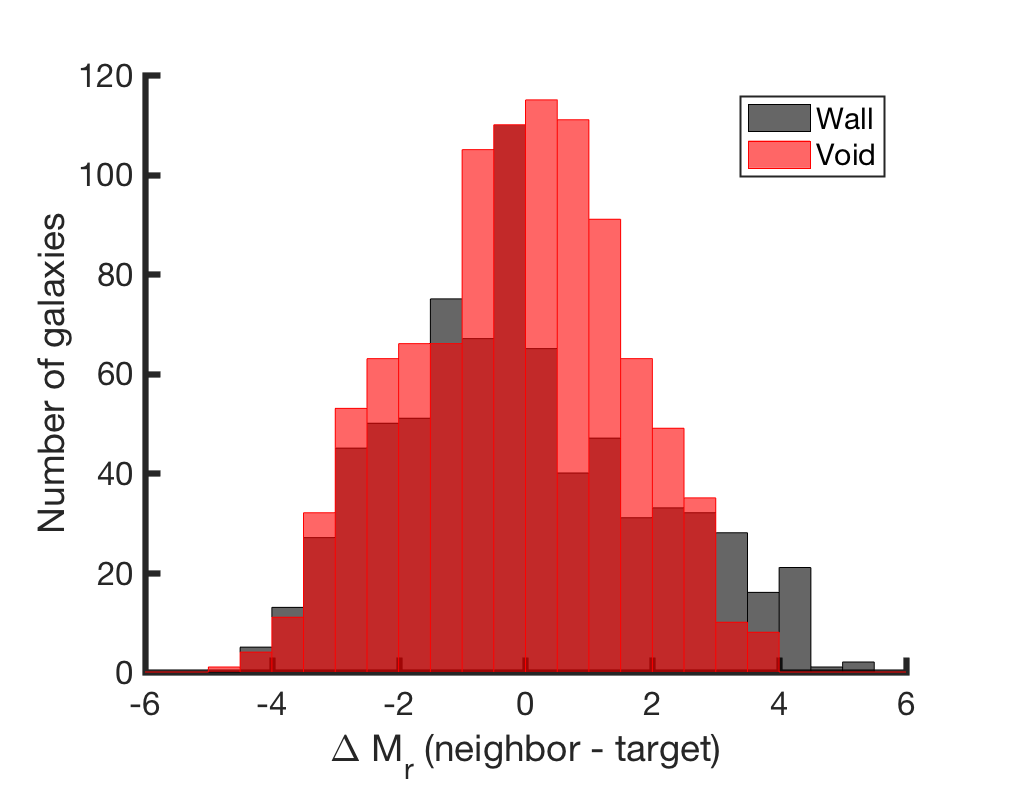
\includegraphics[width=0.49\textwidth]{Images/smallScaleEnvironment/1sig_dwarf_I06relations_Drabsmag_abs_hist}
    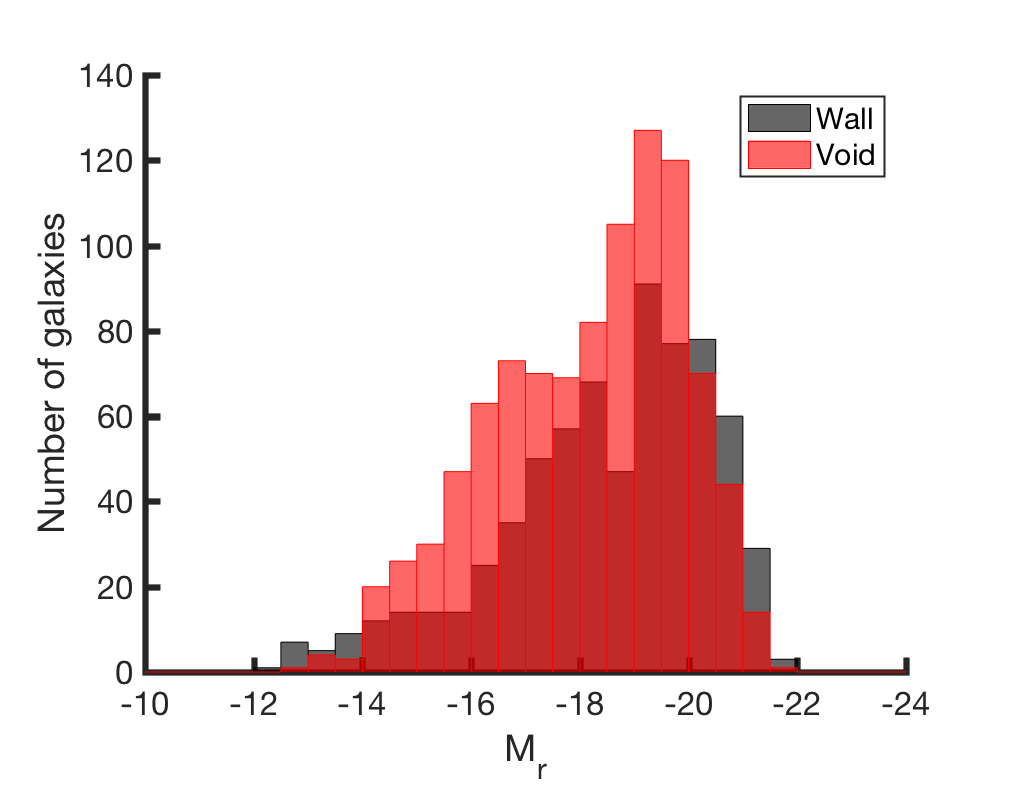
\includegraphics[width=0.49\textwidth]{Images/smallScaleEnvironment/1sig_dwarf_I06relations_rabsmag_vir_hist}
    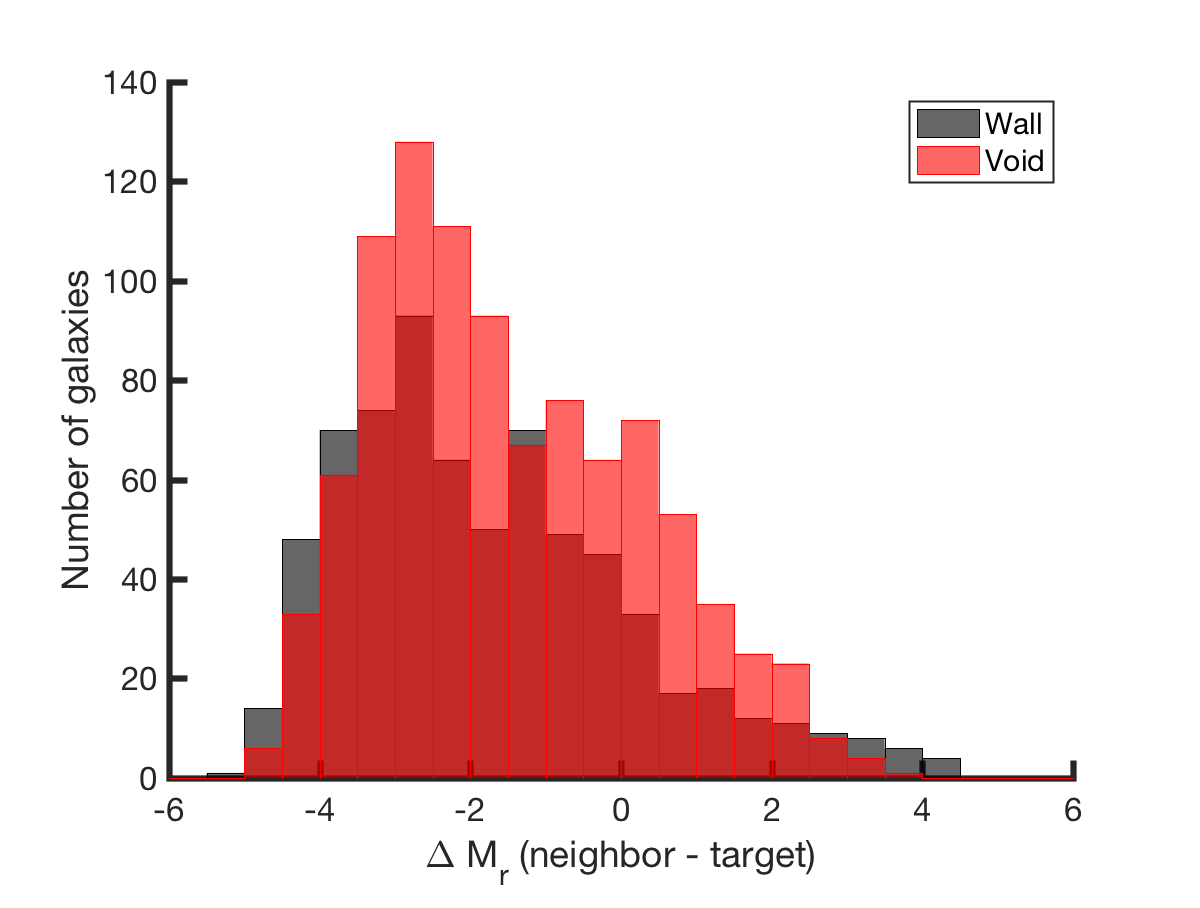
\includegraphics[width=0.49\textwidth]{Images/smallScaleEnvironment/1sig_dwarf_I06relations_Drabsmag_vir_hist}
%    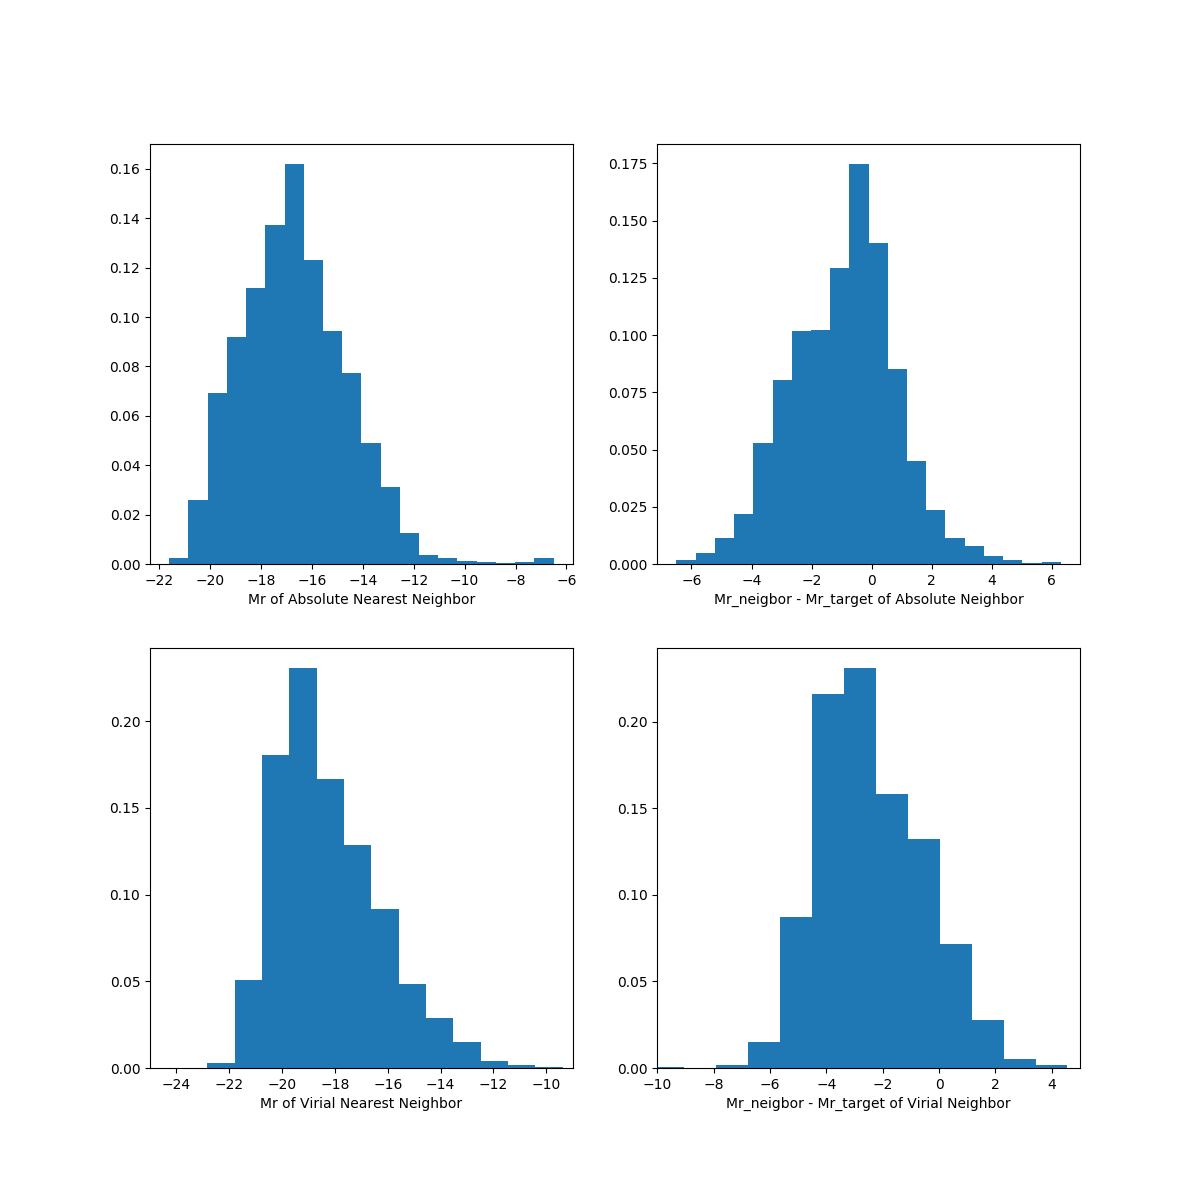
\includegraphics[width=\textwidth]{Images/smallScaleEnvironment/Mr_distribution}
    \caption[Distribution of absolute magnitudes of nearest neighbors]{The 
    distributions in absolute magnitude (left panel) and absolute magnitude 
    relative to the target galaxy (right panel) of the nearest neighbor 
    galaxies.  The top row includes those nearest neighbors in units of \hMpc, 
    and the bottom row consists of the nearest neighbors in units of the 
    neighbor's virial radius.  Comparing the two plots in the right panel, we 
    see that the closest galaxy to the target dwarf galaxies is often of equal 
    or fainter magnitude than the target galaxy.  Alternatively, using the 
    virial radius of the neighbor galaxy as a measure of distance often finds a 
    brighter galaxy than the target galaxy, as the bottom right plot shows.}
    \label{fig:Mr_dist}
\end{figure}

For about 46\% of our dwarf galaxy sample, the two different metrics by which to 
define the nearest neighbor (minimum in units of \hMpc or virial radius of the 
nearest neighbor) return different neighboring galaxies.  Fig. \ref{fig:Mr_dist} 
compares the absolute magnitude distributions of these two nearest neighbor 
populations.  The left panel shows the distribution of the absolute magnitudes 
of the nearest neighbor galaxies, while the right panel shows the distribution 
in absolute magnitude of the nearest neighbor galaxy relative to its target 
galaxy.  The top row includes those nearest neighbors in units of \hMpc, and the 
bottom row consists of the nearest neighbors in units of the neighbor's virial 
radius.  Comparing the two plots in the right panel, we see that the closest 
galaxy to the target dwarf galaxy is often of equal or fainter magnitude than 
the target galaxy.  Alternatively, using the virial radius of the neighbor 
galaxy as a measure of the distance often finds a brighter galaxy than the 
target galaxy, as the bottom right plot in Fig. \ref{fig:Mr_dist} shows.  By 
using these two different distance metrics, we are able to probe the 
relationships between a dwarf galaxy and its nearest neighbor and nearest dark 
matter halo.


\subsection{Including redshift in the distance}
% Evidence of mergers

\begin{figure}
    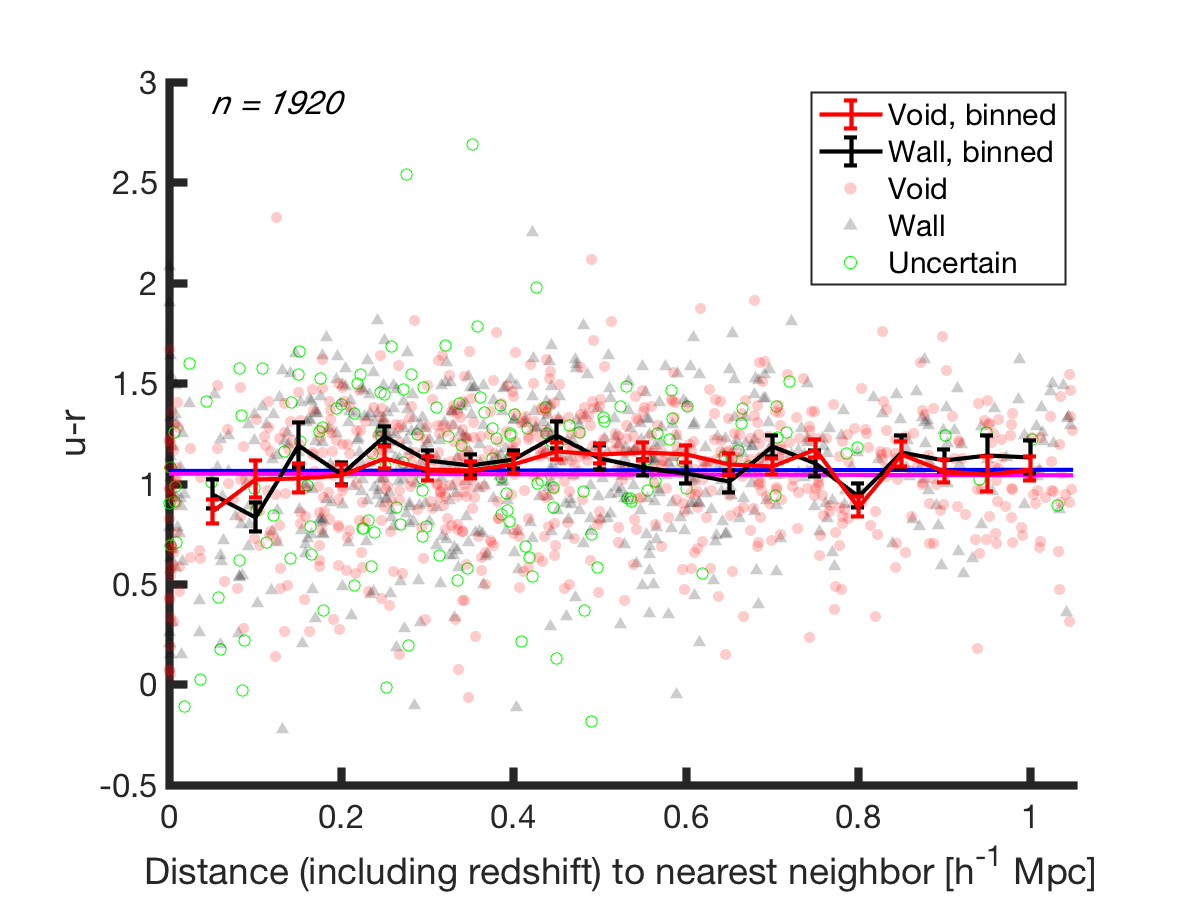
\includegraphics[width=0.49\textwidth]{Images/smallScaleEnvironment/1sig_dwarf_I06relations_zAbsDist_ur}
    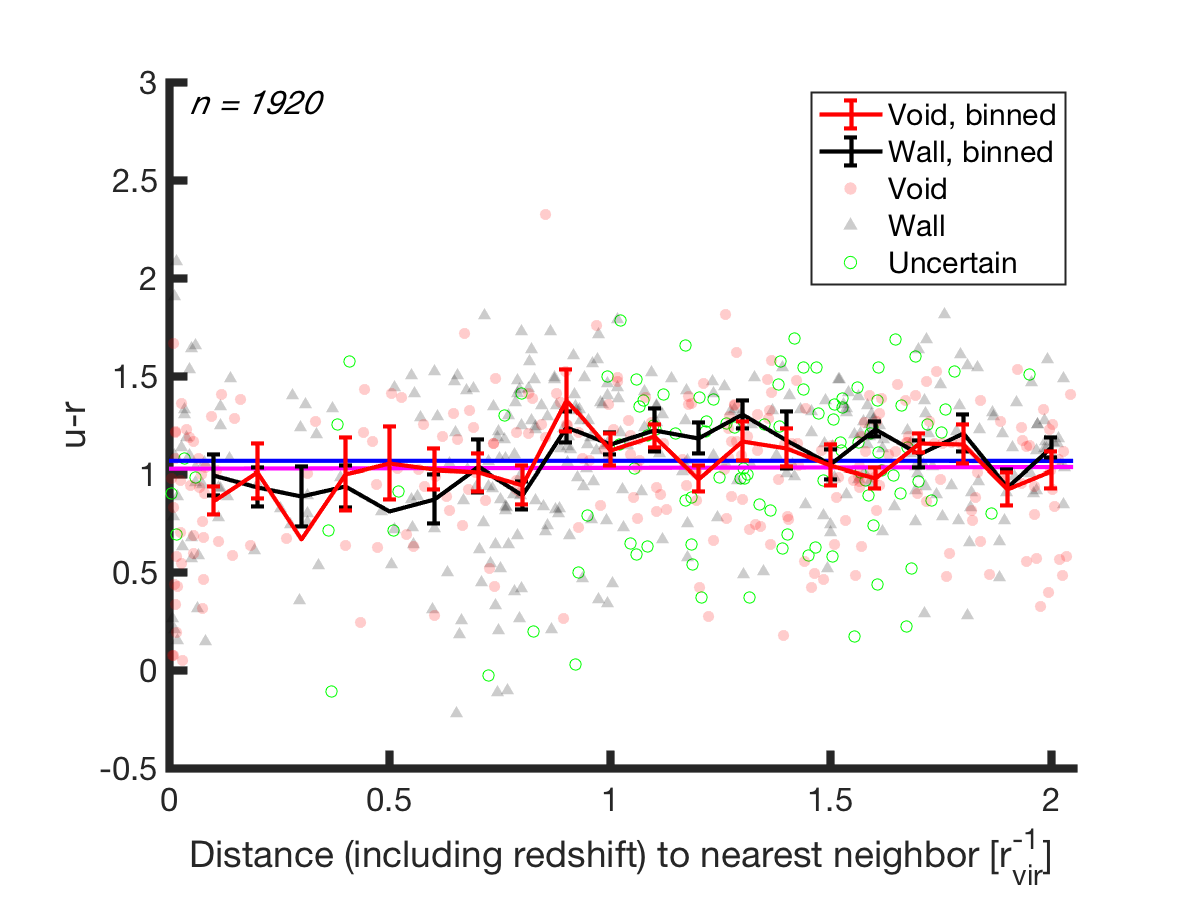
\includegraphics[width=0.49\textwidth]{Images/smallScaleEnvironment/1sig_dwarf_I06relations_zVirDist_ur}
%    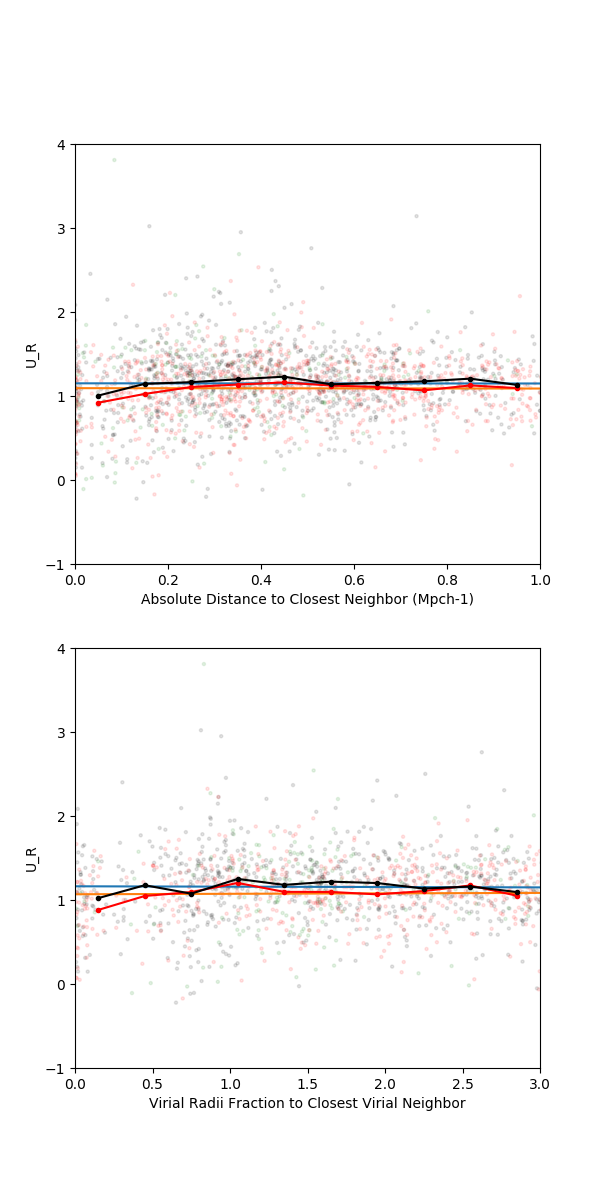
\includegraphics[width=0.5\textwidth]{Images/smallScaleEnvironment/dwarf_ur_xyz}
    \caption[Color versus distance calculated with redshift]{Color versus 
    distance to the nearest galaxy (in units of \hMpc on the left and virial 
    radius on the right) for the star-forming dwarf galaxies.  The redshift is 
    included when calculating the distance to the nearest neighbor.  While there 
    is still no correlation between distance and color, we do note that there is 
    a gap in the distribution of galaxies around a distance of 0.05 \hMpc or 
    0.2$r_{vir}$ from the nearest neighbor.}
    \label{fig:ur_xyz}
\end{figure}

Realizing that the peculiar velocity, which is included in a galaxy's redshift, 
can be significant for galaxies in groups, we have been careful to avoid 
calculating the distance between objects with redshift.  However, we are curious 
to see how the inclusion of redshift in the distance calculations affects the 
results of our analysis.  Therefore, we repeat the same analysis on the 
relationship between color and distance, but this time we include redshift as a 
third component in the distance calculations.  Consequently, we no longer limit 
our sample by a peculiar velocity separation.  Fig. \ref{fig:ur_xyz} shows the 
relationship between these distances and the color of the star-forming dwarf 
galaxies.  When compared to Fig. \ref{fig:ur}, we see that there is no change in 
the correlation between distance and color for the galaxies.  

We note the existence of a gap in the distribution of galaxies around a distance 
of 0.05 \hMpc or 0.2$r_{vir}$ from the nearest neighbor that is not present in 
Fig. \ref{fig:ur}.  When we incorporate the redshift into the distance 
calculations, the resulting distance between galaxies which have small sky 
separations but larger redshift separations is much larger than those with 
larger sky separations and little redshift separation.  As a result, galaxies 
which were originally close to the color axis in Fig. \ref{fig:ur} will be 
moved to much larger distances, while the locations of those which were 
originally further from the color axis will change much less.  The dwarf 
galaxies which remain close to the color axis in Fig. \ref{fig:ur_xyz} must, 
therefore, have small sky separation and almost no difference in their peculiar 
velocities.  We surmise that these represent merging systems, which future 
visual inspection will help to confirm.


%%%%%%%%%%%%%%%%%%%%%%%%%%%%%%%%%%%%%%%%%%%%%%%%%%%%%%%%%%%%%%%%%%%%%%%%%%%%%%%%
%%%%%%%%%%%%%%%%%%%%%%%%%%%%%%%%%%%%%%%%%%%%%%%%%%%%%%%%%%%%%%%%%%%%%%%%%%%%%%%%


\section[Environmental influence]{Small-scale environmental influence}

We see no relationship between a dwarf galaxy's color, sSFR, or gas-phase 
chemical abundances and its distance to the nearest galaxy or group beyond the 
target galaxy's immediate vicinity, implying that the small-scale environment 
($\sim$1 \hMpc) does not significantly influence a dwarf galaxy's evolution.  
This is in contrast to the large-scale environment, which we have seen to 
influence the formation and evolution of dwarf galaxies.

Only those galaxies within 0.05 \hMpc and 0.1$r_{vir}$ (for wall galaxies; 
0.2$r_{vir}$ for void galaxies) of a nearest neighbor appear to deviate from the 
average galaxy values.  The target galaxies within this proximity of their 
nearest neighbor tend to be bluer, have a higher sSFR, and have higher oxygen 
abundances and lower N/O ratios.  Based on the shift in the distribution of 
galaxies seen in Fig. \ref{fig:ur_xyz}, these galaxies might be merging or 
strongly interacting with their nearest neighbor.  If so, this provides evidence 
that galaxy interactions result in a burst of star formation that increases the 
gas-phase chemical abundances of the dwarf galaxies.  Because merging galaxies 
share the same dark matter halo, it appears that the sharing of a dark matter 
halo has more influence on the evolution of a galaxy than the distance to its 
nearest neighbor.

In contrast, dwarf galaxies within 0.05 \hMpc of the center of the nearest group 
have lower oxygen (O/H) and nitrogen (N/H) abundances than average.  Due to 
their proximity to the group center, it is likely that these dwarf galaxies are 
not able to retain as much of their heavy elements as a more isolated galaxy, 
thereby reducing their gas-phase oxygen and nitrogen abundances.


\subsection{Comparison to previous results}

The influence on the gas-phase oxygen abundance within 0.15 \hMpc agrees with 
the results of \cite{Shields91,Pustilnik06,Cooper08,Ellison09,Pustilnik11a,
Pustilnik14}, and \cite{SanchezAlmeida16}, which all find that galaxies with 
higher metallicities preferentially reside in denser regions.  Work by 
\cite{Rupke08} find that interacting galaxies have suppressed metallicities due 
to interaction- or merger-induced gas flows into the galaxy centers.

A study combining the effects of interactions and the large-scale environment is 
presented in \cite{Park09}.  They find two characteristic distances within which 
the behavior of the target galaxy changes: 0.05$r_{vir}$ and $r_{vir}$ of the 
neighboring galaxy.  Our results seem to confirm the significance of distances 
out to 0.05$r_{vir}$, while we see no significant change around the virial 
radius of the neighboring galaxy.  While they only look at galaxies with 
$M_r < -19$ and limit the neighbors to be at least half a magnitude brighter 
than the target, \cite{Park09} find that the morphology and luminosity play a 
significant role in these relationships.  Of particular interest is their 
observation that star formation increases in late type galaxies when their 
nearest neighbor is also of late type.  This is the same behavior we see in our 
sample of dwarf galaxies at distances less than 0.1$r_{vir}$.  With all our 
target galaxies actively forming stars, and more than half of their nearest 
neighbors also dwarf galaxies, it is most likely that our galaxy pairs are also 
of the late-late type.  Based on the results of \cite{Park09}, the deviations we 
see for those galaxies with nearest neighbors within 0.05 \hMpc and 
0.1$r_{vir}$ (for wall galaxies; 0.2$r_{vir}$ for void galaxies) warrant further 
study.


%%%%%%%%%%%%%%%%%%%%%%%%%%%%%%%%%%%%%%%%%%%%%%%%%%%%%%%%%%%%%%%%%%%%%%%%%%%%%%%%
%%%%%%%%%%%%%%%%%%%%%%%%%%%%%%%%%%%%%%%%%%%%%%%%%%%%%%%%%%%%%%%%%%%%%%%%%%%%%%%%


\section{Conclusions}

Using the star-forming dwarf galaxies in the SDSS DR7 sample with gas-phase 
chemical abundances from \cite{Douglass17c}, we investigate the influence of the 
small-scale environment ($\sim 1$ \hMpc) on the evolution of dwarf galaxies.  
From the $\sim$2000 galaxies in the sample, there only appears to be an effect 
from a neighboring galaxy within 0.05 \hMpc or 0.1$r_{vir}$ (for wall galaxies; 
0.2$r_{vir}$ for void galaxies).  The proximity of a group seems to only affect 
the target dwarf galaxy if it is within 0.05 \hMpc.  Thus, the small-scale 
environment does not appear to strongly influence the evolution of dwarf 
galaxies.

We examine the relationship between distance to the nearest neighbor or group 
and the target galaxy's color, sSFR, and gas-phase chemical abundances.  We find 
that, for those galaxies with a neighbor within 0.05 \hMpc or 0.1$r_{vir}$ (for 
wall galaxies; 0.2$r_{vir}$ for void galaxies), the dwarf galaxies are bluer, 
have a higher sSFR, have higher oxygen abundances, and have lower N/O ratios 
than average.  In contrast, dwarf galaxies within 0.05 \hMpc of the center of 
the closest group have lower oxygen and nitrogen abundances.  These results do 
not depend on the maximum peculiar velocity difference, but they may depend on 
the sample (star-forming versus all galaxies).

When we incorporate the redshift into the distance calculations, we find that 
those galaxies within 0.1$r_{vir}$ are most likely mergers or strongly 
interacting with their nearest neighbor.  This matches the results of 
\cite{Park09}, who find that late-late type galaxy pairs within 0.05$r_{vir}$ 
are bluer and have higher star formation rates.  These merging galaxies likely 
share the same dark matter halo, indicating that the dark matter halo is more 
influential on a galaxy's evolution than its distance to the nearest neighbor.

Further analysis of this study should include comparing the properties of the 
target galaxies with the nearest neighbors' properties as a function of 
distance \citep[``galactic conformity'';][]{Weinmann06}.  The gas-phase chemical 
abundances between a galaxy and its nearest neighbor could be strongly 
correlated.